%% (Master) Thesis template
% Template version used: v1.4
%
% Largely adapted from Adrian Nievergelt's template for the ADPS
% (lecture notes) project.


%% We use the memoir class because it offers a many easy to use features.
\documentclass[11pt,a4paper,titlepage]{memoir}

%% Packages
%% ========

%% LaTeX Font encoding -- DO NOT CHANGE
\usepackage[OT1]{fontenc}

%% Babel provides support for languages.  'english' uses British
%% English hyphenation and text snippets like "Figure" and
%% "Theorem". Use the option 'ngerman' if your document is in German.
%% Use 'american' for American English.  Note that if you change this,
%% the next LaTeX run may show spurious errors.  Simply run it again.
%% If they persist, remove the .aux file and try again.
\usepackage[ngerman]{babel}

%% Input encoding 'utf8'. In some cases you might need 'utf8x' for
%% extra symbols. Not all editors, especially on Windows, are UTF-8
%% capable, so you may want to use 'latin1' instead.
\usepackage[utf8]{inputenc}

%% This changes default fonts for both text and math mode to use Herman Zapfs
%% excellent Palatino font.  Do not change this.
\usepackage[sc]{mathpazo}

%% The AMS-LaTeX extensions for mathematical typesetting.  Do not
%% remove.
\usepackage{amsmath,amssymb,amsfonts,mathrsfs}

%% NTheorem is a reimplementation of the AMS Theorem package. This
%% will allow us to typeset theorems like examples, proofs and
%% similar.  Do not remove.
%% NOTE: Must be loaded AFTER amsmath, or the \qed placement will
%% break
\usepackage[amsmath,thmmarks]{ntheorem}

%% LaTeX' own graphics handling
\usepackage{graphicx}

%% We unfortunately need this for the Rules chapter.  Remove it
%% afterwards; or at least NEVER use its underlining features.
\usepackage{soul}

%% This allows you to add .pdf files. It is used to add the
%% declaration of originality.
\usepackage{pdfpages}

%% Some more packages that you may want to use.  Have a look at the
%% file, and consult the package docs for each.
%% See the TeXed file for more explanations

%% [OPT] Multi-rowed cells in tabulars
%\usepackage{multirow}

%% [REC] Intelligent cross reference package. This allows for nice
%% combined references that include the reference and a hint to where
%% to look for it.
\usepackage{varioref}

%% [OPT] Easily changeable quotes with \enquote{Text}
%\usepackage[german=swiss]{csquotes}

%% [REC] Format dates and time depending on locale
\usepackage{datetime}

%% [OPT] Provides a \cancel{} command to stroke through mathematics.
%\usepackage{cancel}

%% [NEED] This allows for additional typesetting tools in mathmode.
%% See its excellent documentation.
\usepackage{mathtools}

%% [ADV] Conditional commands
%\usepackage{ifthen}

%% [OPT] Manual large braces or other delimiters.
%\usepackage{bigdelim, bigstrut}

%% [REC] Alternate vector arrows. Use the command \vv{} to get scaled
%% vector arrows.
\usepackage[h]{esvect}

%% [NEED] Some extensions to tabulars and array environments.
\usepackage{array}

%% [OPT] Postscript support via pstricks graphics package. Very
%% diverse applications.
%\usepackage{pstricks,pst-all}

%% [?] This seems to allow us to define some additional counters.
%\usepackage{etex}

%% [ADV] XY-Pic to typeset some matrix-style graphics
%\usepackage[all]{xy}

%% [OPT] This is needed to generate an index at the end of the
%% document.
%\usepackage{makeidx}

%% [OPT] Fancy package for source code listings.  The template text
%% needs it for some LaTeX snippets; remove/adapt the \lstset when you
%% remove the template content.
\usepackage{listings}
\lstset{
    %language=C++, % We have multiple languages in our thesis
    basicstyle={\normalfont\ttfamily},
    frame=tb,
    framexleftmargin=1.75em,
    xleftmargin=1.75em,
    %xrightmargin=0.25em,
    numbers=left,
    stepnumber=1,
    showstringspaces=false,
    breaklines=true
}

\lstdefinestyle{C++}{
    language=C++,
    keywordstyle=\color{blue},
    stringstyle=\color{red},
    commentstyle=\color{green},
    morecomment=[l][\color{magenta}]{\#}
}

%% [REC] Fancy character protrusion.  Must be loaded after all fonts.
\usepackage{microtype}

%% [REC] Nicer tables.  Read the excellent documentation.
\usepackage{booktabs}

%% \usepackage[a4paper]{geometry}
%% \usepackage{caption}
 \usepackage{subcaption}
%% \usepackage{xcolor}

%% Uncomment for floatbarrier in sections
%\usepackage[section]{placeins}

%% Plots
\usepackage{pgfplots}
%\pgfplotsset{compat=1.8}
%\usepgfplotslibrary{statistics}

%% Filetree
\usepackage{dirtree}

%% Draw diagram
\usetikzlibrary{arrows,positioning,shapes}

%% Disable word-break
%\usepackage[none]{hyphenat}
\hyphenpenalty 10000

%% List spacing
\usepackage{enumitem}
\setlist{nosep}
%\setlist{noitemsep}

%% Our layout configuration.  DO NOT CHANGE.
%% Memoir layout setup

%% NOTE: You are strongly advised not to change any of them unless you
%% know what you are doing.  These settings strongly interact in the
%% final look of the document.

% Dependencies
\usepackage{layout/logo}

% Turn extra space before chapter headings off.
\setlength{\beforechapskip}{0pt}

\nonzeroparskip
\parindent=0pt
\defaultlists

% Chapter style redefinition
\makeatletter

\if@twoside
  \pagestyle{Ruled}
  \copypagestyle{chapter}{Ruled}
\else
  \pagestyle{ruled}
  \copypagestyle{chapter}{ruled}
\fi
\makeoddhead{chapter}{}{}{}
\makeevenhead{chapter}{}{}{}
\makeheadrule{chapter}{\textwidth}{0pt}
\copypagestyle{abstract}{empty}

\makechapterstyle{bianchimod}{%
  \chapterstyle{default}
  \renewcommand*{\chapnamefont}{\normalfont\Large\sffamily}
  \renewcommand*{\chapnumfont}{\normalfont\Large\sffamily}
  \renewcommand*{\printchaptername}{%
    \chapnamefont\centering\@chapapp}
  \renewcommand*{\printchapternum}{\chapnumfont {\thechapter}}
  \renewcommand*{\chaptitlefont}{\normalfont\huge\sffamily}
  \renewcommand*{\printchaptertitle}[1]{%
    \hrule\vskip\onelineskip \centering \chaptitlefont\textbf{\vphantom{gyM}##1}\par}
  \renewcommand*{\afterchaptertitle}{\vskip\onelineskip \hrule\vskip
    \afterchapskip}
  \renewcommand*{\printchapternonum}{%
    \vphantom{\chapnumfont {9}}\afterchapternum}}

% Use the newly defined style
\chapterstyle{bianchimod}

\setsecheadstyle{\Large\bfseries\sffamily}
\setsubsecheadstyle{\large\bfseries\sffamily}
\setsubsubsecheadstyle{\bfseries\sffamily}
\setparaheadstyle{\normalsize\bfseries\sffamily}
\setsubparaheadstyle{\normalsize\itshape\sffamily}
\setsubparaindent{0pt}

% Set captions to a more separated style for clearness
\captionnamefont{\sffamily\bfseries\footnotesize}
\captiontitlefont{\sffamily\footnotesize}
\setlength{\intextsep}{16pt}
\setlength{\belowcaptionskip}{1pt}

% Set section and TOC numbering depth to subsection
\setsecnumdepth{subsubsection}
\settocdepth{subsubsection}

%% Titlepage adjustments
\pretitle{\vspace{0pt plus 0.7fill}\begin{center}\HUGE\sffamily\bfseries}
\posttitle{\end{center}\par}
\preauthor{\par\begin{center}\let\and\\\Large\sffamily}
\postauthor{\end{center}}
\predate{\par\begin{center}\Large\sffamily}
\postdate{\end{center}}

\def\@advisors{}
\newcommand{\advisors}[1]{\def\@advisors{#1}}
\def\@department{}
\newcommand{\department}[1]{\def\@department{#1}}
\def\@thesistype{}
\newcommand{\thesistype}[1]{\def\@thesistype{#1}}

\renewcommand{\maketitlehooka}{\noindent\logo[2in]}

\renewcommand{\maketitlehookb}{\vspace{1in}%
  \par\begin{center}\Large\sffamily\@thesistype\end{center}}

\renewcommand{\maketitlehookd}{%
  \vfill\par
  \begin{flushright}
    \sffamily
    \@advisors\par
    \@department NKSA 
  \end{flushright}
}

\checkandfixthelayout

\setlength{\droptitle}{-48pt}

\makeatother

% This defines how theorems should look. Best leave as is.
\theoremstyle{plain}
\setlength\theorempostskipamount{0pt}

%%% Local Variables:
%%% mode: latex
%%% TeX-master: "thesis"
%%% End:


%% Theorem environments.  You will have to adapt this for a German
%% thesis.
%% Theorem-like environments

%% This can be changed according to language. You can comment out the ones you
%% don't need.

\numberwithin{equation}{chapter}

%% German theorems
%\newtheorem{satz}{Satz}[chapter]
%\newtheorem{beispiel}[satz]{Beispiel}
%\newtheorem{bemerkung}[satz]{Bemerkung}
%\newtheorem{korrolar}[satz]{Korrolar}
%\newtheorem{definition}[satz]{Definition}
%\newtheorem{lemma}[satz]{Lemma}
%\newtheorem{proposition}[satz]{Proposition}

%% English variants
\newtheorem{theorem}{Theorem}[chapter]
\newtheorem{example}[theorem]{Example}
\newtheorem{remark}[theorem]{Remark}
\newtheorem{corollary}[theorem]{Corollary}
\newtheorem{definition}[theorem]{Definition}
\newtheorem{lemma}[theorem]{Lemma}
\newtheorem{proposition}[theorem]{Proposition}

%% Proof environment with a small square as a "qed" symbol
\theoremstyle{nonumberplain}
\theorembodyfont{\normalfont}
\theoremsymbol{\ensuremath{\square}}
\newtheorem{proof}{Proof}
%\newtheorem{beweis}{Beweis}


%% Helpful macros.
%% Custom commands
%% ===============

%% Special characters for number sets, e.g. real or complex numbers.
\newcommand{\C}{\mathbb{C}}
\newcommand{\K}{\mathbb{K}}
\newcommand{\N}{\mathbb{N}}
\newcommand{\Q}{\mathbb{Q}}
\newcommand{\R}{\mathbb{R}}
\newcommand{\Z}{\mathbb{Z}}
\newcommand{\X}{\mathbb{X}}

%% Fixed/scaling delimiter examples (see mathtools documentation)
\DeclarePairedDelimiter\abs{\lvert}{\rvert}
\DeclarePairedDelimiter\norm{\lVert}{\rVert}

%% Use the alternative epsilon per default and define the old one as \oldepsilon
\let\oldepsilon\epsilon
\renewcommand{\epsilon}{\ensuremath\varepsilon}

%% Also set the alternate phi as default.
\let\oldphi\phi
\renewcommand{\phi}{\ensuremath{\varphi}}

%% Highlight single codeword
\newcommand{\codeword}[1]{
    \textcolor{blue}{\lstinline[xleftmargin=5.5em]{#1}}
}

%% Make document internal hyperlinks wherever possible. (TOC, references)
%% This MUST be loaded after varioref, which is loaded in 'extrapackages'
%% above.  We just load it last to be safe.
\usepackage[linkcolor=black,colorlinks=true,citecolor=black,filecolor=black]{hyperref}


% Out packages
% Biblatex for a better bibliography
\usepackage{hyphenat}
\usepackage{array}
\usepackage{caption}
\usepackage{subcaption}
\usepackage[citestyle=numeric, bibstyle=numeric, sorting=none]{biblatex}
\addbibresource{refs.bib}

%% Document information
%% ====================

\title{Nachzeichner KI}
\author{Ian Wasser, Robin Steiner}
\thesistype{Maturarbeit}
\advisors{Betreut durch: Nicolas Ruh}
\date{Oktober 2022}

\begin{document}

\frontmatter

%% Title page is autogenerated from document information above.  DO
%% NOT CHANGE.
\begin{titlingpage}
  \calccentering{\unitlength}
  \begin{adjustwidth*}{\unitlength-24pt}{-\unitlength-24pt}
    \maketitle
  \end{adjustwidth*}
\end{titlingpage}

%% The abstract of your thesis.  Edit the file as needed.
\begin{abstract}
Eine Nachzeicher-KI, die Symbole nachzeichnet
    
\end{abstract}

\newpage
\section*{Vorwort}
Vorwörter

%% TOC with the proper setup, do not change.
\cleartorecto
\begin{KeepFromToc}
\tableofcontents
\end{KeepFromToc}
\mainmatter

%% Template content
%% Some commands used in this file
\newcommand{\package}{\emph}

\chapter{Introduction}

This is version \verb-v1.4- of the template.

We assume that you found this template on our institute's website, so
we do not repeat everything stated there.  Consult the website again
for pointers to further reading about \LaTeX{}.  This chapter only
gives a brief overview of the files you are looking at.

\section{Features}
\label{sec:features}

The rest of this document shows off a few features of the template
files.  Look at the source code to see which macros we used!

The template is divided into \TeX{} files as follows:
\begin{enumerate}
\item \texttt{thesis.tex} is the main file.
\item \texttt{extrapackages.tex} holds extra package includes.
\item \texttt{layoutsetup.tex} defines the style used in this document.
\item \texttt{theoremsetup.tex} declares the theorem-like environments.
\item \texttt{macrosetup.tex} defines extra macros that you may find
  useful.
\item \texttt{introduction.tex} contains this text.
\item \texttt{sections.tex} is a quick demo of each sectioning level
  available.
\item \texttt{refs.bib} is an example bibliography file.  You can use
  Bib\TeX{} to quote references.  For example, read
  \cite{bringhurst1996ets} if you can get a hold of it.
\end{enumerate}


\subsection{Extra package includes}

The file \texttt{extrapackages.tex} lists some packages that usually
come in handy.  Simply have a look at the source code.  We have
added the following comments based on our experiences:
\begin{description}
\item[REC] This package is recommended.
\item[OPT] This package is optional.  It usually solves a specific
  problem in a clever way.
\item[ADV] This package is for the advanced user, but solves a problem
  frequent enough that we mention it. Consult the package's
  documentation.
\end{description}

As a small example, here is a reference to the Section \emph{Features}
typeset with the recommended \package{varioref} package:
\begin{quote}
  See Section~\vref{sec:features}.
\end{quote}


\subsection{Layout setup}

This defines the overall look of the document -- for example, it
changes the chapter and section heading appearance.  We consider this
a `do not touch' area.  Take a look at the excellent \emph{Memoir}
documentation before changing it.

In fact, take a look at the excellent \emph{Memoir} documentation,
full stop.


\subsection{Theorem setup}

This file defines a bunch of theorem-like environments.

\begin{theorem}
  An example theorem.
\end{theorem}

\begin{proof}
  Proof text goes here.
\end{proof}

Note that the q.e.d.\ symbol moves to the correct place automatically
if you end the proof with an \texttt{enumerate} or
\texttt{displaymath}.  You do not need to use \verb-\qedhere- as with
\package{amsthm}.

\begin{theorem}[Some Famous Guy]
  Another example theorem.
\end{theorem}

\begin{proof}
  This proof
  \begin{enumerate}
  \item ends in an enumerate.
  \end{enumerate}
\end{proof}

\begin{proposition}
  Note that all theorem-like environments are by default numbered on
  the same counter.
\end{proposition}

\begin{proof}
  This proof ends in a display like so:
  \begin{displaymath}
    f(x) = x^2.
  \end{displaymath}
\end{proof}


\subsection{Macro setup}

For now the macro setup only shows how to define some basic macros,
and how to use a neat feature of the \package{mathtools} package:
\begin{displaymath}
  \abs{a}, \quad \abs*{\frac{a}{b}}, \quad \abs[\big]{\frac{a}{b}}.
\end{displaymath}

%\chapter{Writing scientific texts in English}

This chapter was originally a separate document written by Reto
Spöhel.  It is reprinted here so that the template can serve as a
quick guide to thesis writing, and to provide some more example
material to give you a feeling for good typesetting.

% We're going to need an extra theorem-like environment for this
% chapter
\theoremstyle{plain}
\theoremsymbol{}
\newtheorem{Rule}[theorem]{Rule}

\section{Basic writing rules}

The following rules need little further explanation; they are best
understood by looking at the example in the booklet by Knuth et al.,
§2--§3.

\begin{Rule}
  Write texts, not chains of formulas.
\end{Rule}

More specifically, write full sentences that are logically
interconnected by phrases like `Therefore', `However', `On the other
hand', etc.\ where appropriate.

\begin{Rule}
  Displayed formulas should be embedded in your text and punctuated
  with it.
\end{Rule}

In other words, your writing should not be divided into `text parts'
and `formula parts'; instead the formulas should be tied together by
your prose such that there is a natural flow to your writing.

\section{Being nice to the reader}

Try to write your text in such a way that a reader enjoys reading
it. That's of course a lofty goal, but nevertheless one you should
aspire to!

\begin{Rule}
  Be nice to the reader.
\end{Rule}

Give some intuition or easy example for definitions and theorems which
might be hard to digest. Remind the reader of notations you introduced
many pages ago -- chances are he has forgotten them. Illustrate your
writing with diagrams and pictures where this helps the reader. Etc.

\begin{Rule}
  Organize your writing.
\end{Rule}

Think carefully about how you subdivide your thesis into chapters,
sections, and possibly subsections.  Give overviews at the beginning
of your thesis and of each chapter, so the reader knows what to
expect. In proofs, outline the main ideas before going into technical
details. Give the reader the opportunity to `catch up with you' by
summing up your findings periodically.

\emph{Useful phrases:} `So far we have shown that \ldots', `It remains
to show that \ldots', `Recall that we want to prove inequality (7), as
this will allow us to deduce that \ldots', `Thus we can conclude that
\ldots. Next, we would like to find out whether \ldots', etc.

\begin{Rule}
  Don't say the same thing twice without telling the reader that you
  are saying it twice.
\end{Rule}

Repetition of key ideas is important and helpful. However, if you
present the same idea, definition or observation twice (in the same or
different words) without telling the reader, he will be looking for
something new where there is nothing new.

\emph{Useful phrases:} `Recall that [we have seen in Chapter 5 that]
\ldots', `As argued before / in the proof of Lemma 3, \ldots', `As
mentioned in the introduction, \ldots', `In other words, \ldots', etc.

\begin{Rule}
  Don't make statements that you will justify later without telling
  the reader that you will justify them later.
\end{Rule}

This rule also applies when the justification is coming right in the
next sentence!  The reasoning should be clear: if you violate it, the
reader will lose valuable time trying to figure out on his own what
you were going to explain to him anyway.

\emph{Useful phrases:} `Next we argue that \ldots', `As we shall see,
\ldots', `We will see in the next section that \ldots, etc.


\section{A few important grammar rules}

\begin{Rule}
  \label{rule:no-comma-before-that}
  There is (almost) \emph{never} a comma before `that'.
\end{Rule}

It's really that simple. Examples:
\begin{quote}
  We assume that \ldots\\
  \emph{Wir nehmen an, dass \ldots}

  It follows that \ldots\\
  \emph{Daraus folgt, dass \ldots}

  `thrice' is a word that is seldom used.\\
  \emph{`thrice' ist ein Wort, das selten verwendet wird.}
\end{quote}
Exceptions to this rule are rare and usually pretty obvious. For
example, you may end up with a comma before `that' because `i.e.' is
spelled out as `that is':
\begin{quote}
  For \(p(n)=\log n/n\) we have \ldots{} However, if we choose \(p\) a
  little bit higher, that is \(p(n)=(1+\varepsilon)\log n/n\) for some
  \(\varepsilon>0\), we obtain that\ldots
\end{quote}
Or you may get a comma before `that' because there is some additional
information inserted in the middle of your sentence:
\begin{quote}
  Thus we found a number, namely \(n_0\), that satisfies equation (13).
\end{quote}
If the additional information is left out, the sentence has no comma:
\begin{quote}
  Thus we found a number that satisfies equation (13).
\end{quote}
(For `that' as a relative pronoun, see also
Rules~\ref{rule:non-defining-has-comma}
and~\ref{rule:defining-without-comma} below.)

\begin{Rule}
  There is usually no comma before `if'.
\end{Rule}

Example:
\begin{quote}
  A graph is not \(3\)-colorable if it contains a \(4\)-clique.\\
  \emph{Ein Graph ist nicht \(3\)-färbbar, wenn er eine \(4\)-Clique
    enthält.}
\end{quote}
However, if the `if' clause comes first, it is usually separated from
the main clause by a comma:
\begin{quote}
  If a graph contains a \(4\)-clique, it is not \(3\)-colorable .\\
  \emph{Wenn ein Graph eine \(4\)-Clique enthält, ist er nicht
    \(3\)-färbbar.}
\end{quote}

There are more exceptions to these rules than to
Rule~\ref{rule:no-comma-before-that}, which is why we are not
discussing them here. Just keep in mind: don't put a comma before `if'
without good reason.

\begin{Rule}
  \label{rule:non-defining-has-comma}
  Non-defining relative clauses have commas.
\end{Rule}
\begin{Rule}
  \label{rule:defining-without-comma}
  Defining relative clauses have no commas.
\end{Rule}

In English, it is very important to distinguish between two types of
relative clauses: defining and non-defining ones. This is a
distinction you absolutely need to understand to write scientific
texts, because mistakes in this area actually distort the meaning of
your text!

It's probably easier to explain first what a \emph{non-defining}
relative clause is. A non-defining relative clauses simply gives
additional information \emph{that could also be left out} (or given in
a separate sentence). For example, the sentence
\begin{quote}
  The \textsc{WeirdSort} algorithm, which was found by the famous
  mathematician John Doe, is theoretically best possible but difficult
  to implement in practice.
\end{quote}
would be fully understandable if the relative clause were left out
completely. It could also be rephrased as two separate sentences:
\begin{quote}
  The \textsc{WeirdSort} algorithm is theoretically best possible but
  difficult to implement in practice. [By the way,] \textsc{WeirdSort}
  was found by the famous mathematician John Doe.
\end{quote}
This is what a non-defining relative clause is. \emph{Non-defining
  relative clauses are always written with commas.} As a corollary we
obtain that you cannot use `that' in non-defining relative clauses
(see Rule~\ref{rule:no-comma-before-that}!). It would be wrong to
write
\begin{quote}
  \st{The \textsc{WeirdSort} algorithm, that was found by the famous
    mathematician John Doe, is theoretically best possible but
    difficult to implement in practice.}
\end{quote}
A special case that warrants its own example is when `which' is
referring to the entire preceding sentence:
\begin{quote}
  Thus inequality (7) is true, which implies that the Riemann
  hypothesis holds.
\end{quote}
As before, this is a non-defining relative sentence (it could be left
out) and therefore needs a comma.

So let's discuss \emph{defining} relative clauses next. A defining
relative clause tells the reader \emph{which specific item the main
  clause is talking about}. Leaving it out either changes the meaning
of the sentence or renders it incomprehensible altogether.  Consider
the following example:

\begin{quote}
  The \textsc{WeirdSort} algorithm is difficult to implement in
  practice. In contrast, the algorithm that we suggest is very simple.
\end{quote}

Here the relative clause `that we suggest' cannot be left out -- the
remaining sentence would make no sense since the reader would not know
which algorithm it is talking about. This is what a defining relative
clause is. \textit{Defining relative clauses are never written with
  commas.} Usually, you can use both `that' and `which' in defining
relative clauses, although in many cases `that' sounds better.

As a final example, consider the following sentence:
\begin{quote}
  For the elements in \(\mathcal{B}\) which satisfy property (A), we
  know that equation (37) holds.
\end{quote}
This sentence does not make a statement about all elements in
\(\mathcal{B}\), only about those satisfying property (A). The relative
clause is \emph{defining}. (Thus we could also use `that' in place of
`which'.)

In contrast, if we add a comma the sentence reads
\begin{quote}
  For the elements in \(\mathcal{B}\), which satisfy property (A), we
  know that equation (37) holds.
\end{quote}

Now the relative clause is \emph{non-defining} -- it just mentions in
passing that all elements in \(\mathcal{B}\) satisfy property (A). The
main clause states that equation (37) holds for \emph{all} elements in
\(\mathcal{B}\). See the difference?


\section[Things you (usually) don't say in English]%
{Things you (usually) don't say in English -- and what to say
  instead}
\label{sec:list}

Table~\ref{tab:things-you-dont-say} lists some common mistakes and
alternatives.  The entries should not be taken as gospel -- they don't
necessarily mean that a given word or formulation is wrong under all
circumstances (obviously, this depends a lot on the context). However,
in nine out of ten instances the suggested alternative is the better
word to use.

\begin{table}
  \centering
  \caption{Things you (usually) don't say}
  \label{tab:things-you-dont-say}
  \begin{tabular}{lll}
    \toprule
    \st{It holds (that) \dots} & We have \dots & \emph{Es gilt \dots}\\
    \multicolumn{3}{l}{\quad\footnotesize(`Equation (5) holds.' is fine, though.)}\\
    \st{$x$ fulfills property $\mathcal{P}$.}& \(x\) satisfies property \(\mathcal{P}\). & \emph{\(x\) erfüllt Eigenschaft \(\mathcal{P}\).} \\
    \st{in average} & on average & \emph{im Durchschnitt}\\
    \st{estimation} & estimate   & \emph{Abschätzung}\\
    \st{composed number} & composite number & \emph{zusammengesetzte Zahl}\\
    \st{with the help of} & using & \emph{mit Hilfe von}\\
    \st{surely} & clearly & \emph{sicher, bestimmt}\\
    \st{monotonously increasing} & monotonically incr. & \emph{monoton steigend}\\
    \multicolumn{3}{l}{\quad\footnotesize(Actually, in most cases `increasing' is just fine.)}\\
    \bottomrule
  \end{tabular}
\end{table}

%%% Local Variables:
%%% mode: latex
%%% TeX-master: "thesis"
%%% End:

%\chapter{Example Chapter}

Dummy text.

\section{Example Section}

Dummy text.

\subsection{Example Subsection}

Dummy text.

\subsubsection{Example Subsubsection}

Dummy text.

\paragraph{Example Paragraph}

Dummy text.

\subparagraph{Example Subparagraph}

Dummy text.

%\chapter{Typography}


\section{Punctuation}

\begin{Rule}
  Use opening (`) and closing (') quotation marks correctly.
\end{Rule}

In \LaTeX, the closing quotation mark is typed like a normal
apostrophe, while the opening quotation mark is typed using the French
\emph{accent grave} on your keyboard (the \emph{accent grave} is the
one going down, as in \emph{frère}).

Note that any punctuation that \emph{semantically} follows quoted
speech goes inside the quotes in American English, but outside in
Britain.  Also, Americans use double quotes first.  Oppose
\begin{quote}
  ``Using `lasers,' we punch a hole in \ldots\ the Ozone Layer,''
  Dr.\ Evil said.
\end{quote}
to
\begin{quote}
  `Using ``lasers'', we punch a hole in \ldots\ the Ozone Layer',
  Dr.\ Evil said.
\end{quote}

\begin{Rule}
  Use hyphens (-), en-dashes (--) and em-dashes (---) correctly.
\end{Rule}

A hyphen is only used in words like `well-known', `$3$-colorable'
etc., or to separate words that continue in the next line (which is
known as hyphenation).  It is entered as a single ASCII hyphen
character (\texttt{-}).

To denote ranges of numbers, chapters, etc., use an en-dash (entered
as two ASCII hyphens \texttt{--}) with no spaces on either side.  For
example, using Equations (1)--(3), we see\ldots

As the equivalent of the German \emph{Gedankenstrich}, use an en-dash
with spaces on both sides -- in the title of Section \ref{sec:list},
it would be wrong to use a hyphen instead of the dash. (Some English
authors use the even longer emdash (---) instead, which is typed as
three subsequent hyphens in \LaTeX. This emdash is used without spaces
around it---like so.)


\section{Spacing}

\begin{Rule}
  \label{rule:no-manual-spacing}
  Do not add spacing manually.
\end{Rule}

You should never use the commands \lstinline-\\- (except within
tabulars and arrays), \lstinline[showspaces=true]-\ - (except to
prevent a sentence-ending space after Dr.\ and such),
\lstinline-\vspace-, \lstinline-\hspace-, etc.  The choices programmed
into \LaTeX{} and this style should cover almost all cases.  Doing it
manually quickly leads to inconsistent spacing, which looks terrible.
Note that this list of commands is by no means conclusive.

\begin{Rule}
  Judiciously insert spacing in maths where it helps.
\end{Rule}

This directly contradicts Rule~\ref{rule:no-manual-spacing}, but in
some cases \TeX{} fails to correctly decide how much spacing is
required.  For example, consider
\begin{displaymath}
  f(a,b) = f(a+b, a-b).
\end{displaymath}
In such cases, inserting a thin math space \lstinline-\,- greatly
increases readability:
\begin{displaymath}
  f(a,b) = f(a+b,\, a-b).
\end{displaymath}

Along similar lines, there are variations of some symbols with
different spacing.  For example, Lagrange's Theorem states that
\(\abs{G}=[G:H]\abs{H}\), but the proof uses a bijection \(f\colon
aH\to bH\).  (Note how the first colon is symmetrically spaced, but
the second is not.)

\begin{Rule}
  Learn when to use \lstinline[showspaces=true]-\ - and
  \lstinline-\@-.
\end{Rule}

Unless you use `french spacing', the space at the end of a sentence is
slightly larger than the normal interword space.

The rule used by \TeX{} is that any space following a period,
exclamation mark or question mark is sentence-ending, except for
periods preceded by an upper-case letter.  Inserting \lstinline-\-
before a space turns it into an interword space, and inserting
\lstinline-\@- before a period makes it sentence-ending.  This means
you should write
\begin{lstlisting}
Prof.\ Dr.\ A. Steger is a member of CADMO\@.
If you want to write a thesis with her, you
should use this template.
\end{lstlisting}
which turns into
\begin{quote}
  Prof.\ Dr.\ A. Steger is a member of CADMO\@.  If you want to write
  a thesis with her, you should use this template.
\end{quote}
The effect becomes more dramatic in lines that are stretched slightly
during justification:
\begin{quote}
  \parbox{\linewidth}{\hbox to \linewidth{%
      Prof.\ Dr.\ A. Steger is a member of CADMO\@.  If you}}
\end{quote}

\begin{Rule}
  Place a non-breaking space (\lstinline-~-) right before references.
\end{Rule}

This is actually a slight simplification of the real rule, which
should invoke common sense.  Place non-breaking spaces where a line
break would look `funny' because it occurs right in the middle of a
construction, especially between a reference type (Chapter) and its
number.


\section{Choice of `fonts'}

Professional typography distinguishes many font attributes, such as
family, size, shape, and weight.  The choice for sectional divisions
and layout elements has been made, but you will still occasionally
want to switch to something else to get the reader's attention.  The
most important rule is very simple.

\begin{Rule}
  When emphasising a short bit of text, use \lstinline-\emph-.
\end{Rule}

In particular, \emph{never} use bold text (\lstinline-\textbf-).
Italics (or Roman type if used within italics) avoids distracting the
eye with the huge blobs of ink in the middle of the text that bold
text so quickly introduces.

Occasionally you will need more notation, for example, a consistent
typeface used to identify algorithms.

\begin{Rule}
  Vary one attribute at a time.
\end{Rule}

For example, for \textsc{WeirdSort} we only changed the shape to small
caps.  Changing two attributes, say, to bold small caps would be
excessive (\LaTeX{} does not even have this particular variation).
The same holds for mathematical notation: the reader can easily
distinguish \(g_n\), \(G(x)\), \(\mathcal{G}\) and \(\mathsf{G}\).

\begin{Rule}
  Never underline or uppercase.
\end{Rule}

No exceptions to this one, unless you are writing your thesis on a
typewriter.  Manually.  Uphill both ways.  In a blizzard.


\section{Displayed equations}

\begin{Rule}
  Insert paragraph breaks \emph{after} displays only where they
  belong.  Never insert paragraph breaks \emph{before} displays.
\end{Rule}

\LaTeX{} translates sequences of more than one linebreak (i.e., what
looks like an empty line in the source code) into a paragraph break in
almost all contexts.  This also happens before and after displays,
where extra spacing is inserted to give a visual indication of the
structure.  Adding a blank line in these places may look nice in the
sources, but compare the resulting display

\begin{displaymath}
  a = b
\end{displaymath}

to the following:
\begin{displaymath}
  a = b
\end{displaymath}
The first display is surrounded by blank lines, but the second is not.
It is bad style to start a paragraph with a display (you should always
tell the reader what the display means first), so the rule follows.

\begin{Rule}
  Never use \lstinline-eqnarray-.
\end{Rule}

It is at the root of most ill-spaced multiline displays.  The
\package{amsmath} package provides better alternatives, such as the
\lstinline-align- family
\begin{align*}
  f(x) &= \sin x, \\
  g(x) &= \cos x,
\end{align*}
and \lstinline-multline- which copes with excessively long equations:
\begin{multline*}
  \def\P{\mathrm P}
  \P\bigl[X_{t_0} \in (z_0, z_0+dz_0],\ldots, X_{t_n}\in(z_n,z_n+dz_n]\bigr]
  \\= \nu(dz_0) K_{t_1}(z_0,dz_1) K_{t_2-t_1}(z_1,dz_2)\cdots
  K_{t_n-t_{n-1}}(z_{n-1},dz_n).
\end{multline*}


\section{Floats}

By default this style provides floating environments for tables and
figures.  The general structure should be as follows:
\begin{lstlisting}
\begin{figure}
  \centering
  % content goes here
  \caption{A short caption}
  \label{some-short-label}
\end{figure}
\end{lstlisting}
Note that the label must follow the caption, otherwise the label will
refer to the surrounding section instead.  Also note that figures
should be captioned at the bottom, and tables at the top.

The whole point of floats is that they, well, \emph{float} to a place
where they fit without interrupting the text body.  This is a frequent
source of confusion and changes; please leave it as is.

\begin{Rule}
  Do not restrict float movement to only `here'
  \textnormal{(\lstinline-h-)}.
\end{Rule}

If you are still tempted, you should avoid the float altogether and
just show the figure or table inline, similar to a displayed equation.

%%% Local Variables:
%%% mode: latex
%%% TeX-master: "thesis"
%%% End:


%% Your real content!
\chapter{Einleitung}\label{chap:einleit}
Der Computer ist ein Werkzeug, das dem Menschen Arbeit abnehmen kann. Um
komplizierte Aufgaben zu übernehmen, muss sich der Computer jedoch an
menschliches Verhalten, menschliches Urteilsvermögen und menschliche Intelligenz
annähern. Mit anderen Worten braucht der Computer, oder das steuernde
Computerprogramm eine künstliche Intelligenz. Es ist schwierig, Intelligenz in
einem Computerprogramm umzusetzen. Der fähigste und am weitesten verbreitete
Ansatz liefert Machine Learning. Diese Arbeit selbst ist eine Untersuchung Im
Bereich Machine Learning. Spezifischer ist die Arbeit im Bereich Reinforcement
Learning, einem Teilgebiet von Machine Learning.

Die Fragestellung der Untersuchung lautet: Kann eine künstliche Intelligenz
lernen, Strichbilder nachzuzeichnen, sodass diese durch ein automatisches System
richtig erkannt werden können?

Für ein gegebenes Strichbild soll die künstliche Intelligenz (KI) erlernen, ein
möglichst gleiches Bild daneben zeichnen können. Die Frage ist, ob die KI das
Nachzeichnen genug gut lernen kann, damit die Zeichnung von einem automatischen
System richtig erkannt wird. Richtig erkannt heisst in diesem Fall vereinfacht,
dass eine zweite KI in der Zeichnung das selbe Motiv wie in der Vorlage erkennt.
Wenn das zutrifft, kann die künstliche Intelligenz erfolgreich nachzeichnen. Es
existieren allerdings weitere Kriterien, die die Leistung der KI bei der
Tätigkeit des Nachzeichnens beurteilen.

Nachzeichnen ist eine menschliche Tätigkeit. Menschen führen beim Zeichnen durch
gewisse Handbewegungen einen Stift, wodurch das Nachzeichnen mit physischen
Einschränkungen verbunden ist. Der Stift kann sich nicht teleportieren, sondern
sich nur mit einer bestimmten Geschwindigkeit fortbewegen. Die KI soll das
Nachzeichnen mit ähnlichen physischen Einschränkungen erlernen. Mit anderen
Worten soll die KI lernen, einen Stift zu führen.  Die
physischen Einschränkungen sind dabei jedoch simuliert und im Vergleich zu der
echten Welt vereinfacht. 

Die KI soll das Nachzeichnen von Strichbildern allgemein erlernen. Strichbilder
können Zahlen, Buchstaben, Formen, Symbole und allgemeine Kritzeleien sein. Die
KI kann nicht mit allen Arten von Strichbildern trainieren, weil die Vielfalt zu
gross ist. Daraus ergibt sich die Frage, wie gut die künstliche Intelligenz
Arten von Strichbildern nachzeichnet, die nicht im Training enthalten waren.

Die vorangehenden Überlegungen sind in einer Sammlung an Unterfragen, die in
dieser Arbeit beantwortet werden, vertreten. Die Unterfragen lauten:
\begin{itemize}
    \item Wie kann die Architektur einer KI aussehen, die das Nachzeichnen erlernt?
    \item Nach welchen Kriterien lässt sich die Leistung der KI in dieser Aufgabe beurteilen?
    \item Wie lässt sich die Leistung der KI in dieser Aufgabe verbessern?
    \item Wie ändert sich die Leistung der KI für Strichbilder, die im Training nicht enthalten sind?
    \item Welche Einflüsse haben physische Einschränkungen auf die Leistungs der KI?
    \item Wie und in wiefern lässt sich die KI mit menschlichem Zeichnen vergleichen?
\end{itemize}



\chapter{Theoretische Grundlagen}\label{chap:t}
Die theoretischen Grundlagen führen die Konzepte ein, die über die ganze Arbeit
hinweg Anwendung finden. Es handelt sich dabei um Zusammenfassungen. Die Theorie
wird auf den Teil reduziert, der für ein grundsätzliches Verständnis der Arbeit
nötig ist. Weitere Informationen werden sind in den referenzierten Quellen
einsehbar. Auch die verwendeten Fachbegriffe werden in diesem Kapitel
eingeführt. 

\section{Machine Learning}\label{chap:t_ml}
Machine Learning ist ein Teilbereich der künstlichen Intelligenz. ``Künstliche
Intelligenz (KI) bezieht sich im Allgemeinen auf jedes menschenähnliche
Verhalten durch eine Maschine oder ein System'' [What is Artificial
Intelligence] Mit Maschinen und Systemen sind in den allermeisten Fällen
Computer, beziehungsweise die steurenden Computerprogramme gemeint. Diese
Computerprogramme bilden ein Modell von menschlichem Verhalten. Machine Learning
Modelle entwickeln (oder erlernen) eine Mustererkennung durch die Analyse von
Daten [What is Machine Learning]. Mustererkennung bedeutet hier, dass der
Algorithmus Zusammenhänge zwischen den analysierten Daten erkennt und auf dieser
Basis Vorhersagen treffen kann. Vereinfacht gesagt, versucht ein Machine
Learning Modell menschliches Urteilsvermögen zu erlernen [is human judgement
necessary].

Ein Beispielproblem für ein Machine Learning Modell ist die Erkennung von
handschriftlichen Zahlen. Ein Computerprogramm soll durch den Input eines Bildes
mit einer handschriftlichen Zahl eine korrekte Beurteilung treffen, um welche
Zahl es sich handelt. Mit anderen Worten soll der Output des Computerprogrammes
der Zahl entsprechen, die auf dem Bild der Eingabe zu sehen ist (siehe autoref{recognition}). Jedes
Computerprogramm, das dieses Problem löst, fällt in den Bereich der künstlichen
Intelligenz. Machine Learning Modelle geben einen Ansatz für die Umsetzung eines
solchen Computerprogrammes.

%todo Bild recognition machine

Machine Learning Modelle, die das Beispielproblem lösen, basieren üblicherweise 
auf Supervised Learning. Das ist ein Teilbereich von Machine Learning, wobei das
Machine Learning Modell aus Rückmeldungen der korrekten Beurteilung, der
Zielvariable, als Reaktion auf ihre eigenen Beurteilungen lernt [datasolut]. Die
Zielvariable muss dabei im Voraus für jeden Datenpunkt in den analysierten Daten
durch einen Menschen festgelegt sein [ML 3.1]. Ausgedrückt durch den Fachbegriff müssen die
Daten labeled sein [2.1 labeled]. Weitere Teilbereiche von Machine Learning sind
Unsupervised Learning und Reinforcement Learning [supervised vs. unsupervised
vs. reinforce]. Beachte \nameref{chap:t_rl} für eine ausgeprägtere Einführung
in Reinforcement Learning.

Machine Learning Modelle sind hauptsächlich in der programmiersprache Python
implementiert [why python]. Dabei werden häufig Tensorflow und Keras verwendet.
Tensorflow ist ein machine Learning Framework [Tensorflow]. Das bedeutet, dass
Tensorflow fertige Funktionen und Algorithmen bereitstellt, die für Machine
Learning Modelle nötig sind. Keras ist ein weiteres Machine Learning Framework,
das selbst mit Tensorflow funktioniert.


\subsection{Funktionsweise eines Machine Learning Modelles}\label{sub:t_ml_func}
Dieser Abschnitt erklärt die Funktionsweise eines Machine Learning Modelles,
basierend auf dem Beispielproblem aus dem letzten Abschnitt (siehe\nameref{chap:t_ml}). 

Bei den Daten, die das Machine Learning Modell analysiert handelt es sich in
diesem Fall um das MNIST Datenset [MNIST]. Dieses Datenset wurde vom NIST
(National Institute of Standards and Technology) in Amerika veröffentlicht und
beinhaltet $70'000$ Bilder von hangeschriebenen Zahlen [NIST EMNIST]. Jedes Bild
hat eine auflösung von $28\times28$ Pixeln (siehe autoref{mnist}).

%todo mnist bild
                
Ein Machine Learning Modell durchläuft ein Training gefolgt von einer Testphase
[Train test split]. Während dem Training erlernt das Modell die Mustererkennung,
um verlässliche Aussagen zu den Daten der Eingabe zu treffen. Die Testphase
misst die Genauigkeit des Modelles, also die Wahrscheinlichkeit, mit der das
Modell die richige Lösung zur Eingabe liefert. Nur in den seltensten Fällen
erreicht diese Genauigkeit $100\%$. Das Modell garantiert somit nicht die
richtige Lösung. Das Machine Learning Modell erlert die Mustererkennung während
dem Training durch die Analyse von Trainingsdaten aus einem Datenset. Das Modell
gibt zu jedem Datenpunkt die Beurteilung, um welche Zahl es sich handelt. Das
Datenset ist labeled (siehe \nameref{chap:t_ml}). Falls die Beurteilung des
Modelles nicht mit der bekannten, korrekten Lösung übereinstimmt, passt sich das
Modell automatisch auf eine bestimmte Weise an. Dadurch soll die Beurteilungen
für zukünftige Datenpunkte genauer werden. Die Testphase misst die Genauigkeit
des Modelles auf Testdaten. Die Testdaten bestehen aus Datenpunkten, die in den
Trainingsdaten nicht enthalten sind.

Zusammengefasst kann Ein Machine Learning Modell Daten Beurteilen und sich
selbst Anpassen, um die Beurteilungen zu verbessern. Künstliche Neuronale Netze
(siehe \nameref{sub:t_ml_nn}) umfassen diese Funktionalität, und finden daher in
Machine Learning Modellen Anwendung.


\subsection{Hyperparameter}\label{sub:t_ml_hyper}
Machine Learning Modelle unfassen verschiedene Hyperparameter. Diese beschreiben
unter anderem wie lange das Training läuft oder wie stark sich das Modell nach
einer falschen Beurteilung anpasst. Diese Hyperparameter beeinflussen das
Lernverhalten des Modelles [Hyperparameter], aber ihr optimaler Wert ist im
Voraus nicht bekannt. 

Hyperparameter können unter anderem durch den Baysian Optimization Algorithmus
optimiert werden [bay Optimization][exploring bayop]. Dieser Algorithmus
versucht, den Output einer Black Box Funktion zu maximieren oder zu minimieren
[bayesopt book s.15]. Eine Black Box ist ein häufig komplexes System, dessen inneren
Vorgänge nicht betrachtet werden [Blackbox Wikipedia]. Bei einer Blackbox
Funktion ist folglich der Input und der Output bekannt, während die Verarbeitung
des Inputs zum Output nicht betrachtet wird (siehe autoref{Blackbox}).

%todo bild Blackbox

Machine Learning Modelle werden häufig als Black Box Funktionen angesehen, da
das Training mit hohem rechnerischen Aufwand verbunden ist, wodurch die genauen
Vorgänge durch einen aussenstehenden Betrachter nicht oder nur schwer erfassbar
sind [how black]. Um ein Machine Learning Modell als eine BlackBox Funktion für
den Baysian Optimization Algorithmus zu verwenden, werden die zu optimierenden
Hyperparameter als Input und eine Zielvariable als Output definiert. Die
Zielvarible des Outputs entspricht dabei einem Wert, der die Leistung des
Modelles widerspiegelt und durch den Algorithmus maximiert werden soll. Ein
Beispiel für die Zielvarible wäre die Genauigkeit des Machine Learning Modelles
(siehe \nameref{sub:t_ml_func}) Die inneren Vorgänge in der BlackBox Funktion
entsprechen in diesem Fall einem Training des Modelles

Der Baysian Optimization Algorithmus kann bis zu 20 Hyperparameter zuverlässig
optimieren [high-dim bay]. Der Algorithmus führt die Blackbox Funktion für eine
bestimmte Anzahl Iterationen mit jeweils verschiedenen Parametern durch. Die
Wahl der Parameter basiert dabei auf Bayes' Theorem [bayesopt book s.7].
Diejenigen Parameter, die den höchsten gefundenen Wert der Zielvariable
auslösen, werden gespeichert.


\subsection{künstliche neuronale Netze}\label{sub:t_ml_nn}
Ein neuronales Netz ist, im biologischen Sinne, "eine beliebige Anzahl Neuronen,
die miteinander Verbunden sind" [Neuro Wikipedia]. Ein Beispiel für ein
neuronales Netz ist das menschliche Gehirn. Künstliche Neuronale Netze
modellieren biologische neuronale Netze in der Form von Programmcode [artificial
neural network]. Diese Arbeit behandelt künstliche neuronale Netze, nicht aber
biologische. Somit handelt es sich bei jedem erwähnten neuronalen Netz, um ein
künstliches neuronales Netz.

Der Grundbaustein eines neuronalen Netzes ist das Neuron. Im Modell stellt das
Neuron ein Objekt dar, das eine beliebiege Anzahl Inputs, aber nur einen Output
hat (siehe autoref{neuron}) [Concept artificial neuron]. Input und Output sind
hierbei rationale Zahlen. Die Ausgabe des Neurons ist im einfachsten Modell, dem
Perzeptron Neuron, grundsätzlich entweder 0 oder 1. Die Ausgabe ist 1, wenn die Summe
der Eingaben einen vorgegebenen Wert, den \emph{Threshold} des Neurons überschreiten.
Ansonsten ist die Ausgabe gleich 0. Jede Eingabe hat ein \emph{Gewicht}, das
einer rationalen Zahl entspricht. Vor der Addition der Inputs wird jeder Input
mit seinem Gewicht multipliziert.  Die Grösse des Gewichts bestimmt somit den
Einfluss der zugehörigen Eingabe auf die Ausgabe des Neurons. [neural networks
deep learning][What is Perceptron]

%todo Bild A neuron

Neuronale Netze in Machine Learning Modellen verwenden kompliziertere Neuronen
als das Perzeptron Neuron, wie zum Beispiel das Sigmoid-Neuron. Die Neuronen
unterscheiden sich in ihrer Activation Function und somit im Verhalten ihres
Outputs [activation function]. So nimmt der Output im Sigmoid-Neuron
beispielsweise auch Werte zwischen $0$ und $1$ an in einem stetigen Übergang
zwischen den beiden Grenzen (siehe autoref{sig vs perc}) [sigmoid Neuron].

%todo Bild sigmoid - perceptron funktion

Neuronale Netze sind Verbindungen dieser Neuronen. Dabei dient die Ausgabe eines
Neurons als eine Eingabe in ein anderes Neuron. Die Neuronen sind in
\emph{Layers} geordnet (siehe autoref{layers}). Neuronale Netze haben mindestens
eine \emph{Input Layer} und eine \emph{Output Layer} [neural network deep
learning][Neural network backprop]. Die Input Layer umfasst die Daten, zu dem das
neuronale Netz eine Beurteilung liefert sollte. Im Beispielproblem (siehe
\nameref{chap:t_ml}) bestände die Eingabe-Ebene aus $28\times28$ Neuronen, wobei
jedes Neuron die Graustufe (durch einen Wert von $0$ bis $255$) eines Pixels im
Bild beschreibt. Der Input ist in diesem Fall zweidimensional. Die Dimensionen
sind allerdings flexibel. Die Output Layer besteht im Beispiel aus $10$
Neuronen, wobei jedes Neuron einer Beurteilung entspricht (das fünfte Neuron
beschreibt zum Beispiel die Ziffer Fünf als Beurteilung). Dasjenige Neuron mit
dem höchsten Output entspricht der Beurteilung des neuronalen Netzes.

%todo Bild Layers

Zwischen der Input Layer und der Output Layers kann es weitere \emph{Hidden
Layers} geben [What are hidden layers]. Es gibt verschiedene Arten von Hidden
Layers, die verschidene Funktionen haben. Zwei der meist verwendeten Layers sind
Fully Connected (Dense) Layers und Convolutional Layers [conv vs. fully
connected]. In Fully Connected Layers dient jedes Neuron als Input für jedes
Neuron in der nächsten Layer. In Convolutional Layers trifft das nicht zu.
(siehe autoref{conv vs. full})Die Funktion von Convolutional Layers ist es,
wichtige Merkmale aus dem Input hervorzuheben [convolutional neural network].
Concatenation Layers [concat] sind eine weitere Form von hidden Layers, die zwei
verschiedene Layers als Input haben und diese somit verbinden. Machine Learning
Modelle werden ab mehr als einer Hidden Layer als Deep Learning Modelle
bezeichnet [deep learning].

%todo Bild conv vs full
%file:///C:/Users/robin/Zotero/storage/PAZJPWRZ/convolutional-layers-vs-fully-connected-layers-364f05ab460b.html

Ein Machine Learning Modell passt während dem Training (siehe
\nameref{sub:t_ml_func}) einzelne Gewichte im neuronalen Netz in der
Hoffnung an, dass die Genauigkeit der Beurteilung mit den angepassten Gewichten
grösser ist. Die Genaue Anpassung erfolgt in den meisten Machine Learning
Modellen durch den Backpropagation Algorithmus [Backpropagation][backpropagation].

\section{Reinforcement Learning}\label{chap:t_rl}
Reinforcement Learning bedeutet Lernen durch Interaktion mit einer Umgebung.
[complete guide]. Genauer gesagt soll ein Machine Learning Modell durch
Rückmeldungen und Beobachtungen aus einer Umgebung ein bestimmtes Verhalten
erlernen.

Reinforcement Learning Modelle führen somit die Umgebung ein. Anders als bei
Supervised Learning und Unsupervised Learning (siehe \nameref{chap:t_ml}) sind
die Daten, aus denen das Modell lernen soll, im Voraus nicht bekannt.
Reinforcement Learning Modelle trainieren somit nicht auf der Grundlage eines
Datensets. Das liegt in der Natur der Umgebung, die häufig zu viele verschiedene
Zustände einnehmen kann, als dass diese in einem Datenset gesammelt werden
könnten. Ein Machine Learning Modell kann trotzdem aus einer Umgebung lernen,
indem es selbst mit dieser interagiert und dadurch Erfahrung sammelt. [synopsis]

Als Beispiel kann die echte Welt als eine Umgebung angesehen werden. Der Mensch
wäre in diesem Fall das Reinforcement Learning Modell. Der Mensch lernt die
Eigenschaften seiner Umgebung durch Interaktionen mit dieser kennen.
Beispielsweise lernt ein Mensch die Schwerkraft durch das Hinfallen kennen.
Durch diese Erfahrungen kann der Mensch ein gewissen Verhalten, zum Beispiel das
Laufen, erlernen. Reinforcement Learning Modelle imitieren dieses Lernverhalten.
So verwendet die Robotik häufig Reinforcement Learning, um einen Roboter laufen
zu lassen. Die Umgebung, mit der das Reinforcement Learning Modell lernt, ist
dabei häufig nicht echt, sondern simuliert.

\subsection{Aufbau und Funktionsweise}\label{sub:t_rl_func}
Dieser Abschnitt umfasst eine genauere Erklärung eines Reinforcement Learning
Modelles, in diesem Fall Deep Q-Learning, unter der Verwendung der korrekten
Fachbegriffe.

Ein Reinforcement Learning Modell umfasst eine \emph{Umgebung} und einen
\emph{Agent}. Der Agent ist dasjenige Element in der Umgebung, welches mit
dieser interagiert und daraus lernt [S.B. s.53]. Die Umgebung verändert sich in
Zeitschritten, genannt \emph{Steps}. In jedem Step führt der Agent eine
\emph{Action} aus, die die Umgebung beeinflusst. Die Entscheidung, welche Action
der Agent ausführt, basiert auf einer \emph{Observation} [DQN s.2] der Umgebung.
Die Observation umfasst alle Daten der Umgebung, die für die Entscheidung des
Agents relevant sind. Der Agent trifft seine Entscheidung auf der Basis eines
neuronalen Netzes (siehe \nameref{sub:t_ml_nn}). Der Input in dieses neuronale
Netz ist die Observation der Umgebung und der Output beschreibt die Action, die
der Agent ausführt. Jedes Neuron des Outputs beschreibt eine spezifische Action
des Agents. Der Agent kann somit nur eine feste Anzahl Actions ausführen. Alle
Actions zusammen werden \emph{Action-Space} [S.B s.67] genannt. Jede Action im
Action-Space besitzt einen \emph{Q-Value}, der dem Output des zugehörigen
Neurons entspricht. (siehe autoref{schema1}) [Q-Learning] Die schlussendliche
Entscheidung, welche Action ausgeführt wird, basiert auf der
\emph{Epsilon-Greedy} Strategie [S.B s.34]. Diese Strategie sieht vor, dass die
Entscheidung mit einer Wahrscheinlichkeit von $\epsilon$ auf eine zufällige
Action fällt. Ansonsten fällt die Entscheidung auf diejenige Action mit dem
höchsten Q-Value. Der Agent erkundet die Umgebung durch die zufälligen Actions,
die er teilweise wählt. Der Agent wählt Actions, die er ansonsten nie wählen
würde, und trifft möglicherweise zufällig auf bessere Optionen für zukünftige
Steps [exploration vs. exploitation]. 

%todo bild reinforcement schema 1

Die Umgebung und somit auch der Agent werden durch die Actions des Agenten
beeinflusst. Dieser Einfluss wird durch die \emph{Reward-Function} gemessen. Die
Reward-Function gibt eine rationale Zahl, den \emph{Reward} aus [S.B s.75]. Umso grösser
der Reward, desto positiver ist der Effekt auf die Umgebung und umgekehrt. Ein
positiver Einfluss auf die Umgebung durch eine Action ist so definiert, dass der
Agent durch die Action das gewünschte Verhalten vorzeigt. Die Reward-Function
definiert, welches Verhalten welchen Reward erzielt. Der Q-Value der gewählten
Action wird mit dem Reward (und dem maximalen Q-Value aus den nächsten möglichen
Actions) addiert. Diese Formel nennt sich Bellman-Gleichung [DQN s.3]. Der neue Q-Value          
nimmt somit einen kleineren Wert an, wenn der Reward negativ ist, und einen
grösseren Wert, wenn der Reward positiv ist. Die Gewichte des neuronalen Netzes
werden daraufhin so angepasst, dass der Output für das Neuron, dessen Action
ausgeführt wurde, näher am neu berechneten Q-Value ist (siehe autoref{schema2}).
Der schlussendliche Effekt ist, dass Actions, die einen positiven Reward
auslösen, wahrscheinlicher gewählt werden, und umgekehrt Actions, die einen
negativen Rewards auslösen, unwahrscheinlicher gewählt werden. Der Agent
versucht insgesamt durch seine Actions einen möglichst hohen akkumulierten
Reward zu erzielen [S.B s.57]. Der akkumulierte Reward entsprich der Summe der
Rewards aus jedem Step.

%todo bild reinforcement schema 2

Das Training läuft in \emph{Episodes} [S.B s.14]. Eine Episode umfasst
eine gewisse Anzahl Steps und am Anfang jeder Episode wird die Umgebung in einen
Startzustand zurückgesetzt. Die Resultate eines Steps werden in dem
\emph{Replay-Buffer} gespeichert. Dazu gehören die Observation der Umgebung, die
Action, und der Reward. Der Replay-Buffer enthält Speicherplatz für eine
bestimmte Anzahl Steps. Während dem Training werden zufällige Steps aus dem
Replay-Buffer gewählt, auf die das neuronale Netz trainiert. Das neurnale Netz
trainiert also auf Daten aus der Vergangenheit der Umgebung und des Agents.
Diese Strategie nennt sich Experience Replay [DQN s.5][DQL]. Ausserdem trainiert
das neuronale Netz jeweils mit einem \emph{Batch} an Steps, also mit einer
gewissen Anzahl an Steps gleichzeitig. Der Replay-Buffer und der Batch sichern
zu, dass das neuronale Netz mit einer grossen Vielfalt an Steps trainiert, was
das Lernverhalten stabiler macht als ein chronologisches Training auf einzelne
Steps [training with exp replay, batch].


\section{Verwandte Arbeiten und Themen}\label{chap:t_ver}
Das Nachzeichnen von Strichbildern hängt allgemein mit dem Zeichnen von Bildern
durch einen Computer zusammen. Es gibt verschiedene Ansätze, um einen Computer
zeichnen zu lassen. Ein häufiger Ansatz ist \emph{Stroke-Based Rendering}
[stroke based rendering]. Stroke-Based Rendering ist das Zeichnen von Bilder
durch das Platzieren von Elementen wie Strichen. Beispiele für Arbeiten in
diesem Bereich sind Strokenet [Strokenet] und ``Learning to Paint With
Model-based Deep Reinforcement Learning'' [learning to paint] Andere Ansätze
simulieren die Führung eines Stiftes. (siehe autoref{stroke-based vs Stift}) Ein
Beispiel dafür ist das Programm Doodle-SDQ [Doodle-SDQ]. Doodle-SDQ beschäftigt
sich auch spezifischer mit dem Nachzeichnen von Strichbildern und wird deswegen
im nächsten Abschnitt weiter behandelt.

%todo bild strokebased vs stife

\subsection{Doodle-SDQ}\label{sub:t_ver_dood}
Doodle-SDQ ist ein Computerprogramm, das durch ein Reinforcement Learning
Modell, spezifischer Deep Q-Learning (siehe \nameref{sub:t_rl_func}), erlernt,
Strichbilder aus dem Google QuickDraw Datenset [Quickdraw Image rec]
nachzuzeichnen. Nachfolgend sind die Aspekte von Doodle-SDQ beschrieben, die für
diese Arbeit relevant sind.

Die QuickDraw Bilder, die das Programm nachzeichnen soll, sind zu einer
einheitliche Grösse von $84\times84$ Pixeln verarbeiteitet [Dood s.7]. Der Agent
kann sich auf einer leeren Zeichenfläche von der selben Grösse bewegen und
zeichnen. Die Umgebung umfasst diese Zeichenfläche, den Agent und das
abzuzeichnende Bild.

Der Agent kann sich durch eine Action in jedem Step auf einen beliebigen Pixel
in einem $11\times11$ Feld, in dessen Zentrum er ist, bewegen. Der Agent kann
ausserdem jede dieser Bewegungen im zeichnenden Zustand oder im nicht
zeichnenden Zustand machen. Der Action-Space hat somit insgesamt eine Grösse von
$2\cdot11\cdot11 = 242$ Actions [Dood s.5]. Im zeichnenden Zustand wird ein Strich auf der
Zeichenfläche zwischen der alten und der neuen Position des Agenten gezeichnet.
Der Agent begeht 100 Steps pro Episode. Eine neue Episdoe entspricht dabei einem
neuen Bild, das abgezeichnet werden soll.

Die Obervation der Umgebung, und somit der Input in das neuronale Netz (siehe
\nameref{sub:t_rl_func}), ist in zwei Teile gegliedert: den Global Stream und
den Local Stream. Der Global Stream hat eine Form von $28\times28\times4$. Der
Input ist somit dreidimensional. Die Form kann als 4 aufeindandergestapelte
Bilder angesehen werden, die jeweils eine Grösse von $28\times28$ Pixeln haben.
Dabei beschreibt eine relle Zahl den Wert von jedem Pixel in einem Bild. Das
erste Bild im global Stream ist die Vorlage, die abgezeichnet werden soll. Das
zweite Bild ist die Zeichenfläche im aktuellen Zustand. Das dritte Bild
beschreibt die Position des Agents durch seine relative Entfernung zu jedem
Punkt auf der Zeichenfläche. Das vierte Bild beschreibt, ob der Agent im
zeichnenden Zustand ist oder nicht. Wenn alle Pixel dieses letzten Bildes den
Wert $1$ haben, ist der Agent im zeichnenden Zustand. Wenn umgekehrt alle Pixel
den Wert $0$ haben, ist der Agent nicht im zeichnenden Zustand. Der Local Stream
hat eine Form von $11\times11\times2$. Er ist somit auch dreidimensional und
beschreibt zwei gestapelte Bilder. Das erste Bild umfasst die Vorlage in dem
$11\times11$ Bereich (bezeichnet als Local image patch [dood s.5]), in dem sich
der Agent in einem Schritt bewegen kann. Das zweite Bild beschreibt den selben
Bereich von der Zeichenfläche [Dood s.4 f.]. Der global Stream und der Local
Stream werden durch eine Concatenation Layer (siehe \nameref{sub:t_ml_nn})
zusammengeführt.

Die Reward-Function (siehe \nameref{sub:t_rl_func}) bezieht sich auf die
Differenz der Anzahl der übereinstimmenden Pixel zwischen der Vorlage und
Zeichenfläche zwischen zwei Steps [Dood s.6]. Eine grosse Menge an neu
übereinstimmenden Pixel entsprechen somit einem höheren Reward als wenige neu
übereinsimmende Pixel. Wenn nach einem Step weniger Pixel übereinstimmen als
zuvor, entspricht das einem negativen Reward. 

\section{Git und GitHub}\label{chap:t_git} Git und Github sind weit verbreitete
Hilfsmittel für Software Entwickler. Git ist ein Programm, während GitHub ein
Service ist, der dieses Programm in der Cloud zugänglich macht. GitHub hat
zusätzliche Funktionen, die die Zusammenarbeit zwischen mehreren Entwicklern
erleichtern. Die genaue Funktion und das Zusammenspiel dieser beiden Hilfsmittel
wird nachfolgend erläutert.

\subsection{Git}\label{sub:t_git_git}
Git erkennt Veränderungen im Code eines Projektes und speichert diese
Veränderungen in einer neuen Version ab. Die einzelnen Versionen des Projektes
bleiben dabei zu jedem Zeitpunkt abrufbar. Dieses Konzept nennt sich Version
Control [Version Control]. Das Programm wurde 2005 von Linus Torvald entwickelt
[Git]. Versionen des Projektes werden manuell durch einen Commit gespeichert. Es
wird empfohlen, nur jeweils ein bestimmtes Problem oder eine bestimmte Funktion
pro Commit anzugehen [Git best practic]. Für grössere Funktionen oder Probleme
kann ein Branch erstellt werden. Ein Branch ermöglicht eine abgekapselte
Entwicklung eines Projektes [Git Branch]. Zum Beispiel kann das Projekt in
mehreren Branches gleichzeitig und unabhängig von einander entwickelt werden.
Das übliche Vorgehen mit Branches sieht so aus, dass aus einem Main Branch für
jede grössere Funktion ein Branch erstellt wird (siehe autoref{branch
structure}). Die Entwicklung der Funktion findet nur in dem zugehörigen Branch
statt. Erst wenn die Funktion fertig ist, wird der Branch wieder mit dem Main
Branch zusammengeführt. Wenn die Arbeit in einem Branch scheitert, kann dieser
gelöscht werden, ohne den Main Branch zu beeinflussen [Git How Branch].

%todo bild branch structure

\subsection{GitHub}\label{sub:t_git_gh}
GitHub wurde 2008 von Chris Wanstrath, PJ Hyett, Scott Chacon und Tom
Preston-Werner entwickelt \cite{noauthor_github_2021}. 2018 wurde das
Unternehmen von Microsoft gekauft. GitHub ist ein Service, der Projekte, die mit
Git verwalten werden, in der Cloud speichert. Dadurch kann ein Projekt überall
und von beliebig vielen Personen entwickelt werden. GitHub betreibt eine
Webseite, über welche der Service verwendet werden kann
\cite{noauthor_github_2021}.

GitHub besitzt verschiedene Hilfsmittel, die die Zusammenarbeit von Entwicklern
weiter vereinfachen. Beispiele dafür sind Issues und Project Boards. Diese
Hilfsmittel ermöglichen Organisation, Strukturierung und Arbeitsteilung. Ein
weiteres Hilfsmittel sind Pull Requests. Eine Pull Reqeust wird dann gestellt,
wenn die Arbeit an einem Branch fertig ist. Durch Pull Requests können die
Entwickler des Projektes die Funktionalität eines Branches überprüfen. Wenn ein
Branch nicht die gewünschte Aufgabe erfüllt, kann die Pull Request abgelehnt
werden. Erst wenn eine Pull Request angonommen wird, kann der Branch wieder in
den Main Branch zurückgeführt werden [Pull Request].


\chapter{Methode}\label{chap:m}
Die Methode dieser Untersuchung besteht darin, die in der Fragestellung
beschriebene künstliche Intelligenz (KI) zu entwickeln und dessen Leistung
auszuwerten. Die Diskussion dieser Resultate führt schlussendlich zu einer
Antwort auf die Fragestellung. Die Entwicklung der KI besteht aus zwei Teilen.
Der eine Teil umfasst die Definition der Kriterien, nach denen die Leistung der
KI evaluiert wird (siehe \doubleref{chap:m_eval}). Der andere Teil umfasst die
Entwicklung der KI (siehe \doubleref{chap:m_grund}), zusammen mit verschiedenen
Variationen davon (siehe \doubleref{chap:m_var}). Die Variationen haben jeweils
einen unterschiedlichen Fokus auf die definierten Kriterien. Die Auswertung
(siehe \doubleref{chap:m_auswert}) der Leistung der KI bezieht sich ebenfalls
auf die definierten Kriterien.

\section{Grundprogramm}\label{chap:m_grund} Die KI ist abhängig von den
Kriterien, die dessen Leistung definieren (siehe \doubleref{chap:m_eval}). Mit
anderen Worten trainiert die KI auf diese Kriterien. Das Ziel des
Grundprogrammes ist, die allgemeine Trainingsumgebung für die KI
bereitzustellen. Dieses Grundprogramm ist unabhängig von einem spezifischen
Kriterium und ermöglicht das Training auf ein beliebiges Kriterium.
Reinforcement Learning Modelle mit einer undefinierten Reward Function (siehe
\doubleref{sub:t_rl_func}) umfassen diese Eigenschaften. Das Grundprogramm ist
in Python unter der Verwendung des Keras Frameworks implementiert (siehe
\doubleref{chap:t_ml}). 

\subsection{Doodle-SDQ als Basis}\label{sub:m_grund_dood} Das Reinforcement
Learning Modell des Grundprogrammes basiert auf Doodle-SDQ (siehe
\doubleref{sub:t_ver_dood}). Von Doodle-SDQ ist das neuronale Netz, bezogen auf
die Form des Inputs, des Outputs und den Hidden Layers, grösstenteils
übernommen. Die relevanten Anpassungen zwischen Doodle-SDQ und dem Grundprogramm
dieser Arbeit sind nachfolgend erläutert.

Bei der Umgebung handelt es sich, wie bei Doodle-SDQ, um eine Zeichenfläche,
worauf sich der Agent bewegt. Das Grundprogramm wird auf das
Nachzeichnen von Ziffern trainiert. Die Ziffern stammen aus dem MNIST Datenset
(siehe \doubleref{chap:t_ml}) und haben somit eine Grösse von $28\times28$
Pixeln. Die Fläche, worauf sich der Agent bewegen   
kann, hat folglich auch eine Grösse von $28\times28$ Pixeln. Der Global Stream
(siehe \doubleref{sub:t_ver_dood}) des Inputs in das Neuronale Netz ändert sich
bis auf die neue Grösse der Bilder nicht. Die Pixel der Bilder, wie auch die
Zeichenfläche, nehmen den Wert von einem Bit an. Eine Null repräsentiert einen
schwarzen (nicht gezeichneten) Pixel an dieser Stelle im Bild und eine Eins
einen weissen (gezeichneten) Pixel. Die genaue Architektur des neuronalen Netzes
ist im Schema \autoref{fig:architecture} angegeben.

%Bild architecture
\begin{figure}[!ht]
  \centering
  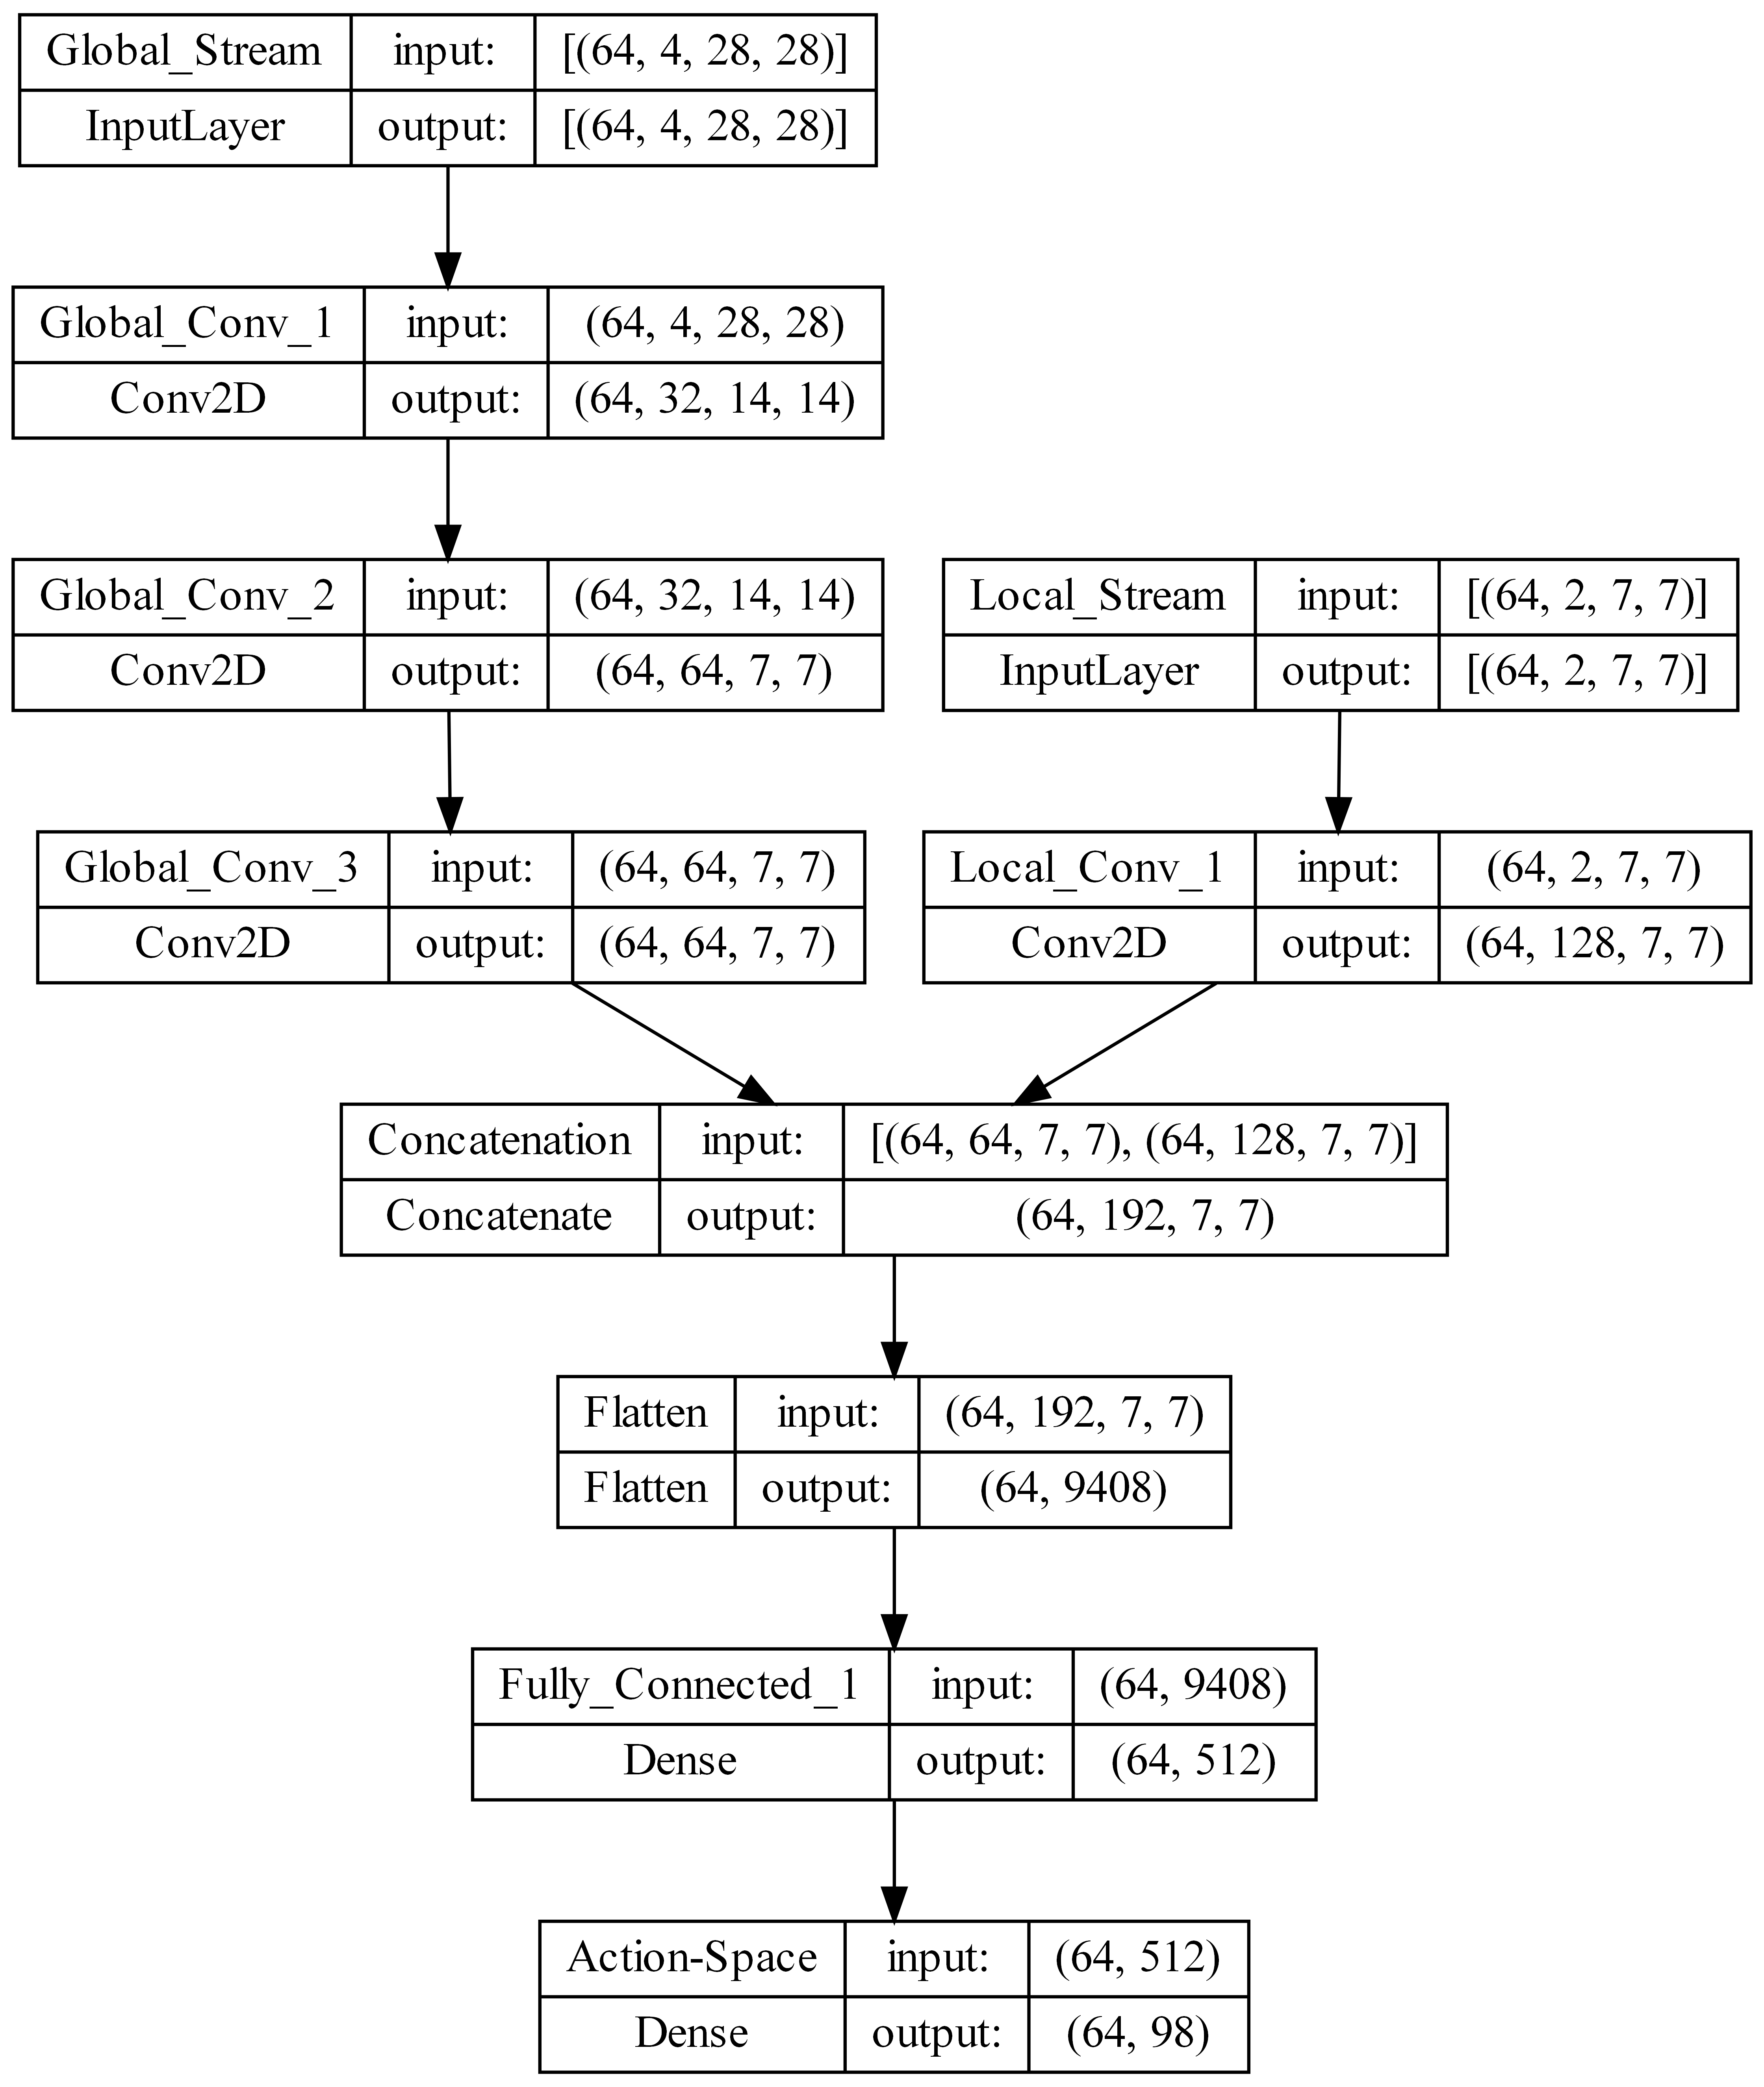
\includegraphics[width=\textwidth-2cm]{images/methode/architecture.png}
  \caption{Architektur des neuronalen Netzes im Grundprogramm (eigene Abbildung, mit Keras erstellt) Jeder Block repräsentiert einen Layer. Die Form des Inputs und des Outputs ist von jedem Layer angegeben}
  \label{fig:architecture}
\end{figure}

Der Local Stream und damit auch der Local image Patch schrumpfen von $11\times11$
Pixel auf $7\times7$ Pixel. Somit schrumpft gleichzeitig der Action-Space (siehe
\doubleref{sub:t_rl_func}) des Agenten von $2\cdot11\cdot11 = 242$ Actions auf
$2\cdot7\cdot7 = 98$ Actions. Das bedeutet für den Agent, dass er sich pro Step
um maximal drei Pixel von seiner Position wegbewegen kann. Diese Bewegung kann
der Agent entweder zeichnend oder nicht zeichnend ausführen (siehe
\autoref{fig:actionspace}).

%bild normal actionspace
\begin{figure}[!ht]
  \centering
  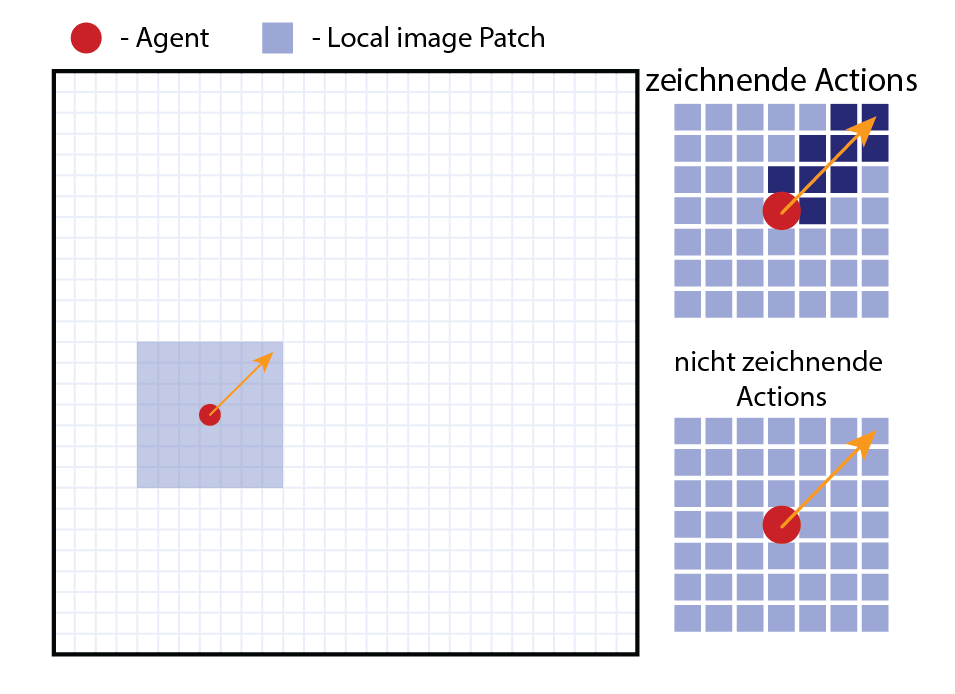
\includegraphics[width=\textwidth]{images/methode/actionspace.png}
  \caption{Action-Space im Grundprogramm}
  \label{fig:actionspace}
\end{figure}

Falls der Agent die Action zeichnend ausführt, zieht das Programm einen Strich
zwischen der alten und der neuen Position. Mit anderen Worten werden alle Pixel
der Zeichenfläche zwischen den beiden Positionen weiss. Der Strich hat eine
festgelegte Breite von $3$ Pixeln. Am Anfang jeder Episode, also mit jeder neuen
Ziffer, startet der Agent in einer zufälligen Position im nicht zeichnenden
Zustand. Am Anfang jeder Episode ist die Zeichenfläche leer, also vollkommen
Schwarz.

Actions des Agents, die ihn über die vorgegebene Zeichenfläche hinaus
positionieren würden, sind nicht zulässig. Diese Actions können vom Agent nicht
gewählt werden und ihr optimaler Q-Value (siehe \doubleref{sub:t_rl_func}) ist
in jedem Fall $0$. Das hat zur Folge, dass nach dem Training die allermeisten
unzulässigen Actions einen Q-Value nahe oder gleich $0$ haben. Das senkt die
Wahrscheinlichkeit, dass der Agent versucht, eine unzulässige Action
auszuführen.

\subsection{Präparierung der Daten und Optimierung}\label{sub:m_grund_data}
Die Trainingsdaten bestehen aus $36'000$ Bildern von handgeschriebenen Ziffern
aus dem MNIST Datenset (siehe \doubleref{chap:t_ml}). Die restlichen Bilder des
MNIST Datensets machen die Testdaten aus. Die Bilder im Datenset sind als Bitmap
dargestellt, wobei jedes Element (jeder Pixel) einen Wert zwischen $0$ und $255$
annimmt. Die Zahl repräsentiert eine Graustufe, wobei $0$ Schwarz ist und $255$
Weiss. Diese Graustufen werden entfernt. Jeder Pixel mit einem Wert über $0$
übernimmt den Wert $1$, wodurch die Bilder nur noch aus Einsen und Nullen
bestehen. Dabei ist $0$ Schwarz und $1$ Weiss (siehe \autoref{fig:norm-v-nogray}).
So stimmen die Bilder mit den Zeichnungen, die der Agent produzieren kann,
überein.

%Bild normal num vs nogray num
\begin{figure}[!ht]
  \centering
  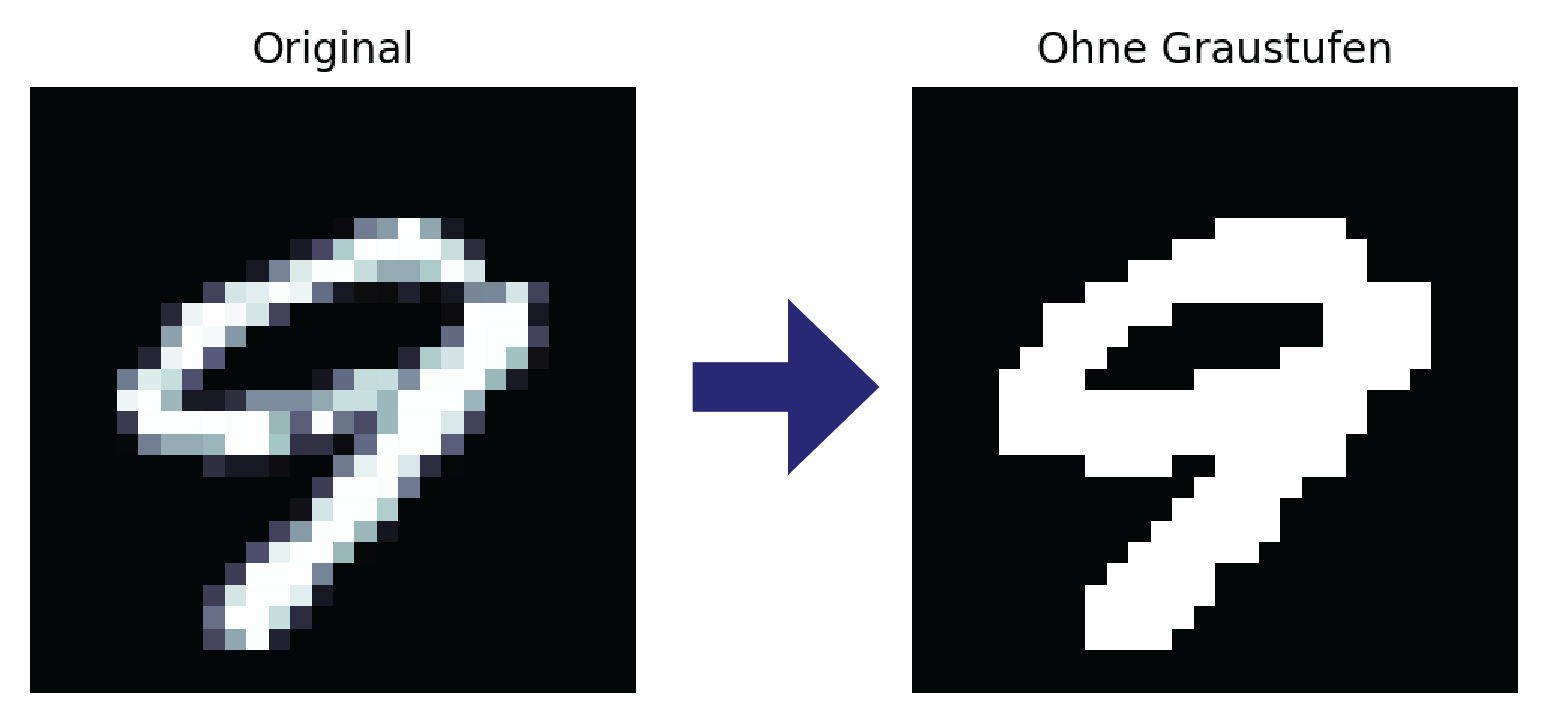
\includegraphics[width=\textwidth]{images/methode/norm-v-nogray.png}
  \caption{Entfernung der Graustufen im MNIST Datenset (eigene Abbildung)}
  \label{fig:norm-v-nogray}
\end{figure}


Das Grundprogramm trainiert mit $3'000$ Bildern, von denen jede Ziffer $300$
Bilder ausmacht. Die restlichen Bilder in den Trainingsdaten sind für mögliche  
Erweiterungen aufgehoben. Der Agent zeichnet jedes der $3'000$ Bilder ein Mal und
trainiert somit für $3'000$ Episodes. Die Der Agent zeichnet für $64$ Steps pro
Episode.

Die Hyperparameter des Grundprogrammes, wie auch die der Variationen (siehe
\doubleref{chap:m_var}) sind durch den Bayesian Optimization Algorithmus
optimiert (siehe \doubleref{sub:t_ml_hyper}). Die Implementierung des
Algorithmus in Python stammt von \cite{fernando_nogueira_bayesian_2014}. Der
Algorithmus ändert sich für verschiedene Variationen der KI nicht und ist somit
Teil des Grundprogrammes. Mit jeder Iteration des Baysian Optimization
Algorithmus trainiert das Reinforcement Learning Modell für eine vom Algorithmus
selbst bestimmte Anzahl Episodes. Die Zielvariable, die durch den Baysian
Optimization Algorithmus maximiert werden soll, wird am Ende jeder Iteration des
Trainings in der Testumgebung berechnet (siehe \doubleref{sub:m_auswert_test}).
Auf welchem der drei Kriterien (siehe \doubleref{chap:m_eval}) die Zielvariable
basiert, ist frei wählbar.



\section{Evaluation der Leistung}\label{chap:m_eval}
In diesem Unterkapitel sind die Kriterien definiert, welche die Leistung der
künstlichen Intelligenz evaluieren. Mit anderen Worten beschreiben die
Kriterien, wie gut die KI nachzeichnet. Für eine präzise und objektive
Evaluation sind alle Kriterien durch einen Zahlenwert repräsentiert. Die
Kriterien und ihre jeweilige Berechnung werden nachfolgend beschrieben.

\subsection{Erkennbarkeit}\label{sub:m_eval_rec}
Das Kriterium der Erkennbarkeit beschreibt, ob in der Vorlage das gleiche Motiv
wie in der Zeichnung der künstlichen Intelligenz erkannt wird. Wenn
Beispielsweise in beiden Fällen eine Fünf erkannt wird, hat das Kriterium den
Wert $1$. Wird in der Vorlage eine Fünf erkannt, aber in der Zeichnung eine
Vier, hat das Kriterium den Wert $0$

Das erkannte Motiv wird durch eine zweite KI beurteilt (siehe
\doubleref{sub:t_ml_func}). Diese zweite KI beurteilt ein Motiv nur als erkannt,
wenn das zugehörige Neuron im Output des neuronalen Netzen einen Wert von über
$0.75$ hat. Das entspricht laut dem neuronalen Netz mit einer hohen
Wahrscheinlichkeit der korrekten Beurteilung.

Um die verschiedenen Arten von Strichbildern, die die KI zeichnen soll, zu
erkennen, existieren vortrainierte Machine Learning Modelle. Die in dieser
Arbeit implementierten vortrainierten Modelle sind in der \autoref{tab:models}
ersichtlich. Diese Modelle sind mit den selben Daten trainiert, die in der
Testumgebung (siehe \doubleref{sub:m_auswert_test}) als Vorlage zum Abzeichnen
dienen.

\begin{table}[!ht]
  \centering
  \begin{tabular}{|l|l|l|l|}
  \hline
      Art & Entwickler & Trainiert mit \\ \hline
      Ziffern & \cite{mazzia__2022} & MNIST \\ \hline
      Buchstaben & \cite{mor_emnist_2022} & EMNIST Letters \\ \hline
      \makecell{Strichbilder\\von Objekten} & \cite{lam_linus_keras_2022} & Auswahl aus QuickDraw \\ \hline
  \end{tabular}
  \caption{Vortrainierte Modelle}
  \label{tab:models}
\end{table}

\subsection{Prozentuale Übereinstimmung}
\label{sub:m_eval_proc}
Dieses Kriterium beschreibt die prozentuale Übereinstimmung der weissen
(gezeichneten) Pixel zwischen der Vorlage und der Zeichnung der KI (siehe
\doubleref{chap:m_grund}). Der Wert $K$ dieses Kriteriums zu dem Step $t$
berechnet sich aus folgender Formel:
\[ K(t) = \frac{G(t)}{G_{\max}} \] $G_{\max}$ entspricht der Anzahl aller
weissen Pixeln in der Vorlage. $G(t)$ entspricht der Anzahl der weissen Pixel,
die zwischen der Vorlage und der Zeichenfläche übereinstimmen. Die Pixel, die
nicht übereinstimmen, zählen negativ für $G(t)$. $G(t)$ und somit auch $K(t)$
können dadurch auch negative Werte annehmen. Der maximale Wert von $K(t)$ ist 1,
was einer prozentualen Übereinstimmung von $100\%$ entspricht (siehe
\autoref{fig:ubereinstimmung}).

%bild übereinstimmung
\begin{figure}[!ht]
  \centering
  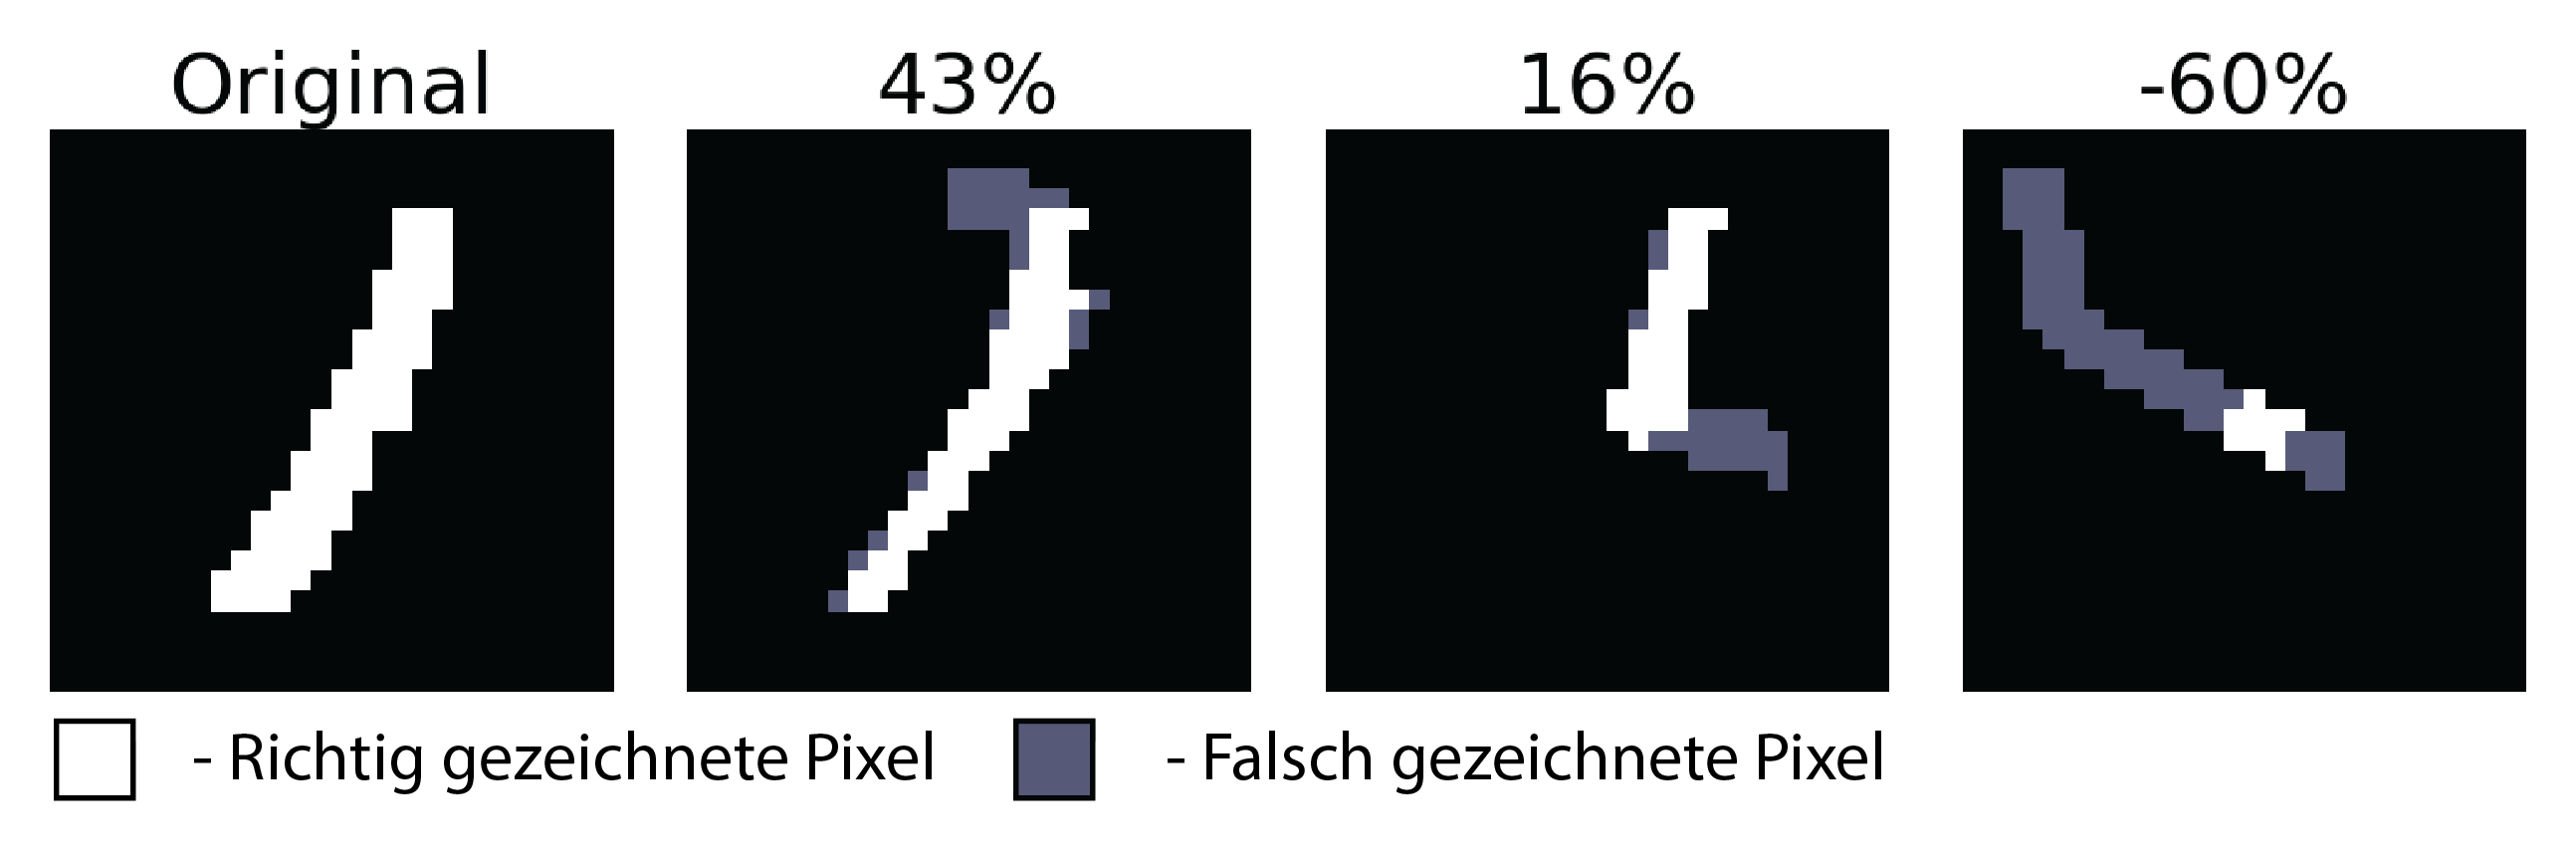
\includegraphics[width=\textwidth]{images/methode/ubereinstimm.png}
  \caption{Drei Beispiele für den Wert des Kriteriums der Übereinstimmung (eigene Abbildung)}
  \label{fig:ubereinstimmung}
\end{figure}

\subsection{Geschwindigkeit}\label{sub:m_eval_speed}
Dieses Kriterium beschreibt, wie schnell die Zeichnung der KI fertig ist. Der
Wert dieses Kriteriums entspricht der Anzahl Steps bis zur Fertigstellung der
Zeichnung. Eine kleinere Anzahl Steps entspricht einer schnelleren Fertigstellung
der Zeichnung und somit einer besseren Leistung bezogen auf dieses Kriterium.

Eine Zeichnung gilt als fertig, wenn die prozentuale Übereinstimmung (siehe
\doubleref{sub:m_eval_proc}) mindestens $70\%$ beträgt und die Zahl der
Definition entsprechend erkannt wird (siehe \doubleref{sub:m_eval_rec}). Wenn
die Zeichnung bis zum Ende der Episode die Bedingungen einer fertigen Zeichnung
nicht erfüllt, hat dieses Kriterium den Wert $64$. Das entspricht der Anzahl
Steps, die von der KI pro Episode insgesamt begangen werden (siehe
\doubleref{sub:m_grund_data}).


\section{Variationen}\label{chap:m_var}
Dieses Unterkapitel beschreibt verschiedene Variationen, ausgehend vom
Grundprogramm (siehe \doubleref{chap:m_grund}). Bei einigen dieser Variationen
handelt es sich um konkrete Implementierungen der definierten Kriterien in die
Reward-Function (siehe \doubleref{sub:t_rl_func}). Die Reward-Function kann
dabei auf mehreren Kriterien gleichzeitig basieren. Der Unterschied zwischen den
Variationen liegt im Fokus auf die Kriterien. Einige Variationen sind
untereinander kombinierbar, andere Variationen führen strukturelle Veränderungen
für die KI ein, die über die Reward-Function hinaus gehen.

\subsection{Basis Reward-Function}\label{sub:m_var_base}
Die Basis Reward-Function ist die einfachste Erweiterung des Grundprogrammes
(siehe \doubleref{chap:m_grund}). Diese Reward-Function implementiert das
Kriterium der prozentualen Übereinstimmung (siehe \doubleref{sub:m_eval_proc}).
Der Reward für eine Action berechnet sich aus der Differenz zwischen der
prozentualen Übereinstimmung vor dem Ausführen der Action, und der prozentualen
Übereinstimmung nach dem Ausführen der Action (also $K(t-1)$ und $K(t)$). Somit
wird der Reward $R$ zum Step $t$ durch folgende Formel berechnet. 
\[ R(t) = K(t) - K(t-1) \] Der Reward eines Steps entspricht folglich nicht der
gesamten prozentualen Übereinstimmung zu einem Step. Stattdessen Entspricht der
Reward der Veränderung der prozentualen Übereinstimmung, ausgelöst durch die
Action in einem Step. Der akkumulierte Reward (siehe \doubleref{sub:t_rl_func})
enstspricht dem absoluten Wert der prozentualen Übereinstimmung.


\subsection{Training auf Geschwindigkeit}\label{sub:m_var_speed}
Das Kriterium der Geschwindigkeit (siehe \doubleref{sub:m_eval_speed}) kann in
die Reward-Function integriert werden. Dadurch trainiert die künstliche
Intelligenz auf eine minimale Zeit bis zur Fertigstellung der Zeichnung. Die
Variation verwendet grundsätzlich die Basis Reward-Function (siehe
\doubleref{sub:m_var_base}). Die vorgeschlagene Anpassung davon sieht
folgendermassen aus: Am Ende jeder Episode wird der Reward jedes Steps in der
Episode mit einem Faktor $f$ multipliziert. Dieser Faktor berechnet sich aus
folgender Formel:
\[ f = 2 - \frac{S}{S_{\max}} \] 
$S_{\max}$ entspricht der Anzahl Steps, die der Agent in einer Episode begeht
(siehe \doubleref{sub:m_grund_data}). $S$ entspricht der Anzahl Steps bis zur
Fertigstellung der Zeichnung. Der Faktor nimmt einen Wert zwischen $1$ und $2$
an. Ein grosser Faktor $f$ entspricht einem hohen Reward und wird durch eine
schnelle Fertigstellung der Zeichnung ausgelöst. Wenn der Agent die Zeichnung
bis zum Ende einer Episode nicht fertigstellt, ist $f = 1$. In diesem Fall unterscheidet sich die
Reward-Function nicht von der Basis Reward-Function. Wenn die Zeichnung früher
fertiggestellt wird, zeichnet der Agent trotzdem alle $S_{\max}$ Steps. Das
verhindert eine ungleichmässige Verteilung zwischen verschiedenen Episodes im
Replay-Buffer (siehe \doubleref{sub:t_rl_func}). In diesem Fall wird $S$
allerdings nur in dem Step gespeichert, in dem die Zeichnung zum ersten Mal die
Bedingung einer Fertigstellung erfüllt.   

Indem das Kriterium der Geschwindigkeit während dem Training angepasst wird,
verstärkt sich der Fokus auf auf eine möglichst schnelle Fertigstellung. Die
minimale prozentuale Übereinstimmung einer fertigen Zeichnung ist als $75\%$
definiert. Zu beginn des Trainings wird dieser Wert auf $25\%$ heruntergesetzt,
und über das Training hinweg linear bis auf $75\%$ erhöht. Dadurch löst die
Reward Function bei einer unfertigen Zeichnung bereits positive Rewards für die
Geschwindigkeit aus. Für diese Anpassung wird Die Bedingung der korrekten
Erkennung (siehe \doubleref{sub:m_eval_speed}) nicht beachtet.


\subsection{Training auf Erkennbarkeit}
\label{sub:m_var_rec}
Das Kriterium der Erkennbarkeit kann, anders als die anderen Kriterien, nur
teilweise in die Reward Function integriert werden. Das Kriterium strebt eine
Erkennbarkeit, unabhängig von der Art der Strichbilder, an (siehe
\doubleref{sub:m_eval_rec}). Die künstliche Intelligenz trainiert allerdings nur
auf das Nachzeichnen von Ziffern. Aus diesem Grund trainiert diese Variation nur
auf die Erkennbarkeit von Ziffern, und lässt die anderen Arten von Strichbildern
aussen vor. 

Die Reward-Function (siehe \doubleref{sub:t_rl_func}) dieser Variation beinhaltet
eine zweite KI, die handgeschriebene Ziffern erkennt (siehe
\autoref{tab:models}). Diese zweite KI beurteilt in jedem Step, welche
Ziffern sie in der Vorlage und in der aktuellen  %TODO Code präzision
Zeichnung erkennt

Die einfachste Form der Reward-Function für diese Variation sähe
folgendermassen aus: Wenn eine Zeichnung das Kriterium der Erkennbarkeit
erfüllt, löst die Reward Function einen Reward von $0.05$. In diesem Zustand
funktioniert die Reward-Function allerdings nicht. Der Agent kann den
akkumulierten Reward nicht maximieren. Zwei Ansätze gehen auf dieses Problem
ein. Beide Ansätze sind Teil dieser Variation.

Der erste Ansatz schlägt vor, die zweite KI erst ab einer gewissen prozentualen
Übereinstimmung (siehe \doubleref{sub:m_eval_proc}) einzusetzen. In diesem Fall
löst die korrekte Erkennung erst ab einer prozentualen Übereinstimmung von
$20\%$ einen positiven Reward aus. Diese zusätzliche Bedingung ist notwendig,
weil die Beurteilungen der zweiten KI teilweise für einen menschlichen
Betrachter fragwürdig sind. Zum Beispiel schätzt die zweite KI eine leere
Zeichenfläche mit einer hohen Sicherheit als eine Eins ein (siehe
\autoref{fig:wrong-minst-rec}). Das ist ein Problem, weil dadurch der Agent
einen positiven Reward für eine leere Zeichenfläche erhält. Das stört das
weitere Lernverhalten, weil es die Wahrscheinlichkeit erhöht, dass die KI nicht
mehr zeichnet.

% Bild falsche mnist rec
\begin{figure}[!ht]
  \centering
  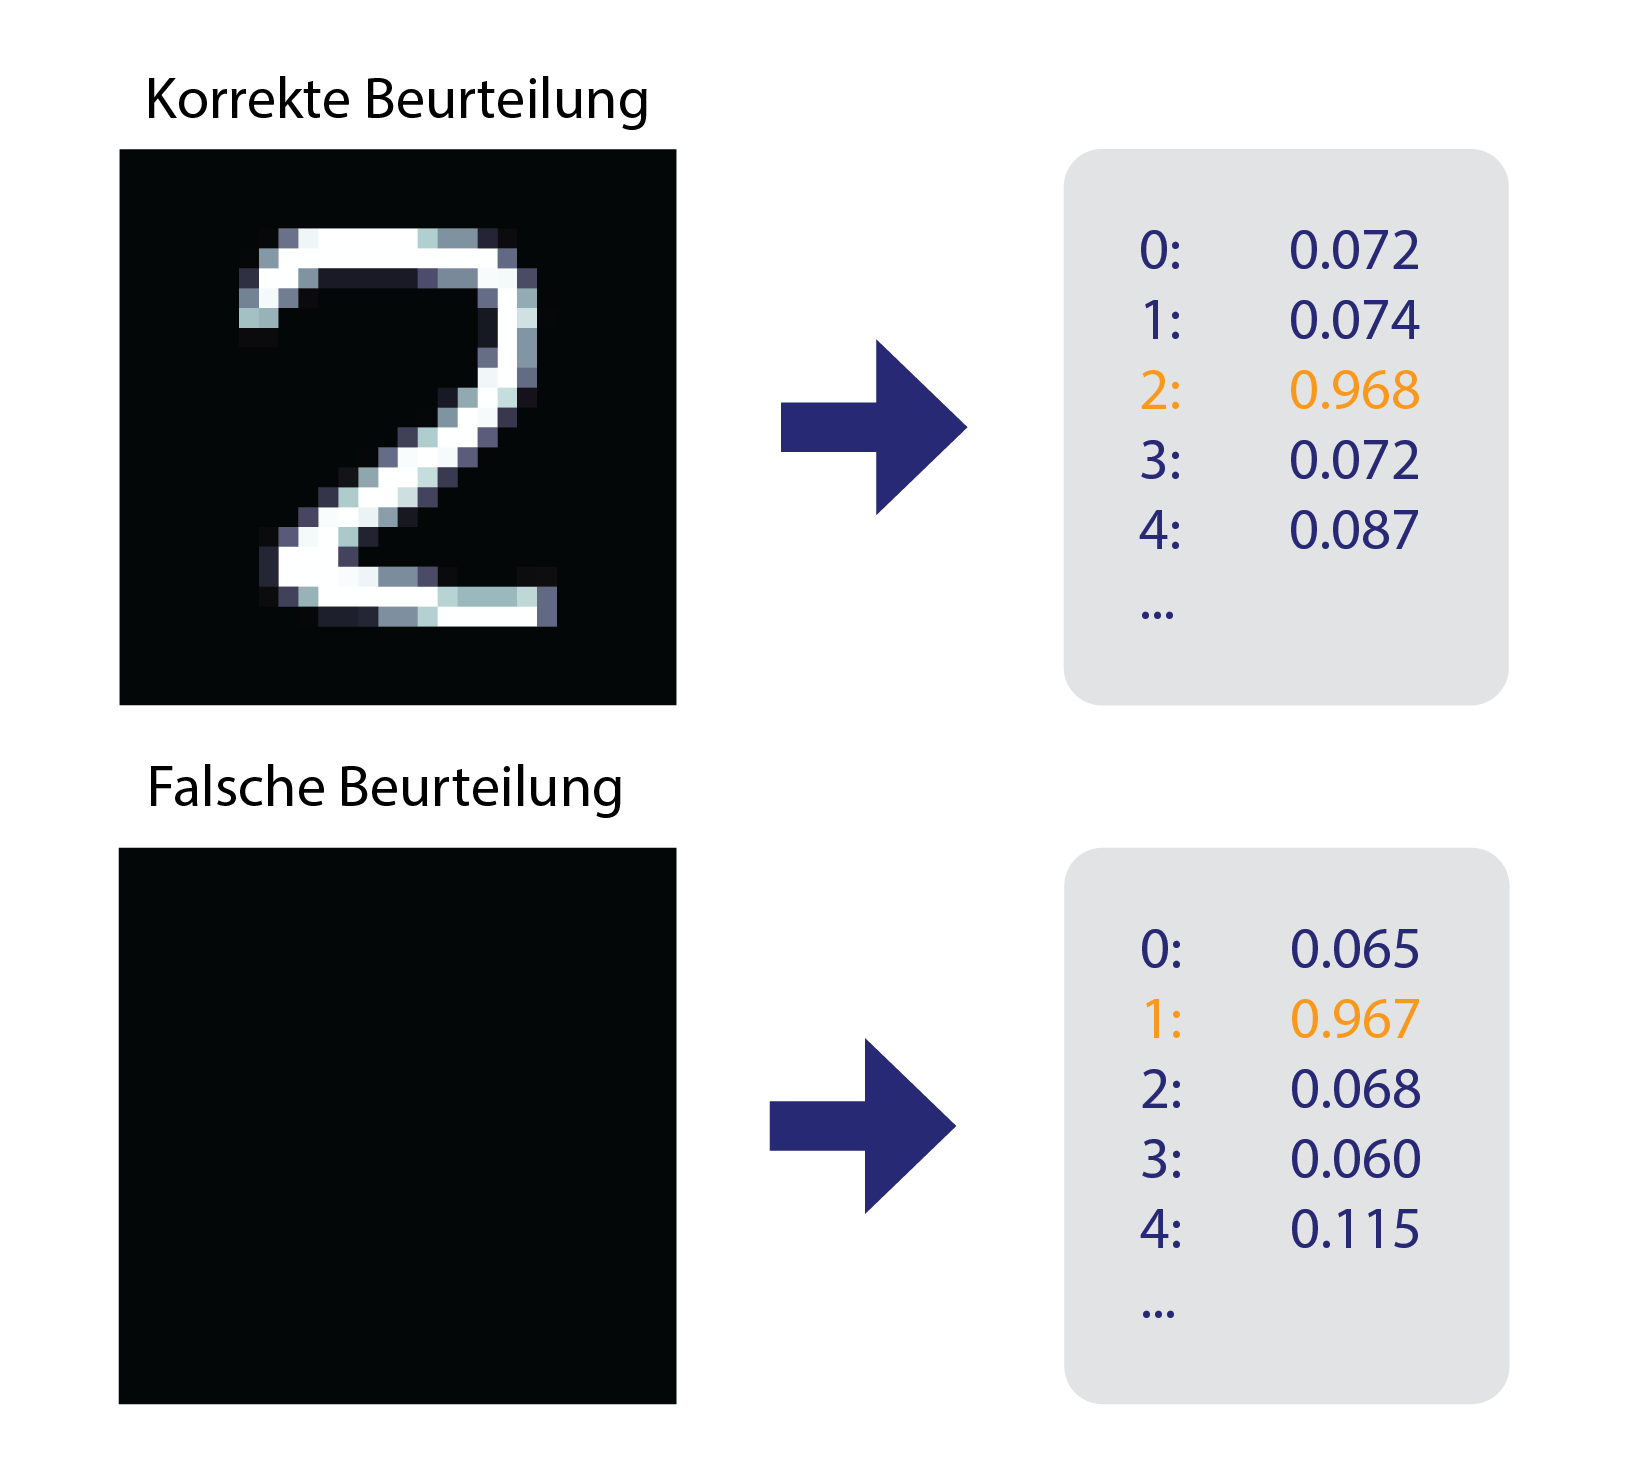
\includegraphics[width=\textwidth]{images/methode/wrong-mnist-rec.png}
  \caption{Beispiele einer richtigen und einer falschen Erkennung von handgeschriebenen Zahlen durch eine KI (eigene Abbildung). Die Werte sind durch einen Test der KI berechnet }
  \label{fig:wrong-minst-rec}
\end{figure}

Der zweite Ansatz implementiert neben der Reward-Function der Erkennbarkeit
erneut die Basis Reward-Function (siehe \doubleref{sub:m_var_base}). Die Relevanz
der beiden Reward-Functions ändert sich allerdings über das Training hinweg. Die
Rewards werden in jedem Step mit einem bestimmten Faktor multipliziert. Zu
Beginn des Trainings ist der Faktor für den Reward der Basis Reward-Function
$f_b = 1$ und der Faktor für den Reward basierend auf der Erkennbarkeit $f_e =
0$. Vom Start ausgehend sinkt $f_b$ linear und $f_e$ steigt linear. Ab einem
gewissen Punkt bleiben beide Faktoren stehen (siehe \autoref{fig:decrementor}).
Blieben die Faktoren ab diesem Punkt nicht konstant, würde die Variation,
gestützt auf Beobachtungen, an der Stabilität ihrer Leistung verlieren.

% Bild Decrementor
\begin{figure}[!ht]
  \centering
  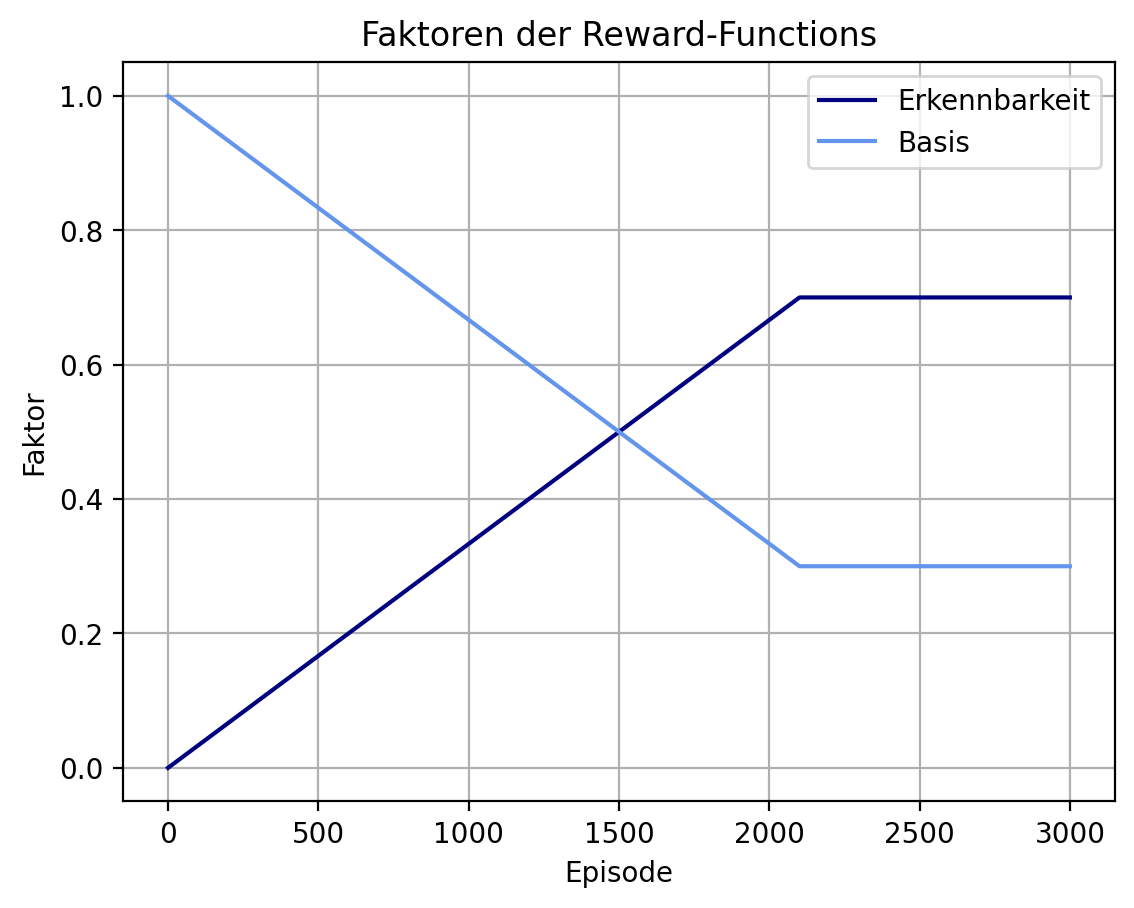
\includegraphics[width=\textwidth-2cm]{images/methode/decrementor.png}
  \caption{Veränderung der Faktoren der Basis Reward-Function und der Reward-Function der Erkennbarkeit über das Training hinweg (eigene Abbildung)}
  \label{fig:decrementor}
\end{figure}

Das Zusammenspiel der beiden Reward-Functions hat den Vorteil, dass die
künstliche Intelligenz zu Beginn des Trainings durch die Basis Reward-Function
für kleine Erfolge positive Rewards erzielt. Die Reward-Function der
Erkennbarkeit ermöglicht das nicht, da sie erst für eine korrekte Erkennung
einen Reward auslöst. Eine Korrekte Erkennung ist allerdings für eine
untrainierte KI schwer zu erreichen. Gewissermassen wird die KI durch die Basis
Reward-Function vortrainiert, um schlussendlich mit der Reward-Function der
Erkennbarkeit effizient trainieren zu können.


\subsection{Physikalische Umgebung}\label{sub:m_var_phy}
Diese Variation spezialisiert sich auf kein Kriterium. Stattdessen verändert
sich die Umgebung, in der sich der Agent bewegt (siehe
\doubleref{sub:t_rl_func}). Auch der Input und der Output des neuronalen Netzes
sind angepasst. Durch diese Veränderungen löst sich die Variation vom
Grundprogramm. Sie bleibt allerdings mit den anderen Variationen kompatibel, Da
diese ausschliesslich die Reward-Function anpassen.

Die Variation ergänzt die Umgebung durch physikalische Simulationen. Diese
physikalische Umgebung definiert die physischen Rahmenbedingungen des Zeichnens
neu, mit dem Ziel, diese näher an die Realität zu bringen.

Der Agent hat neu eine Geschwindigkeit, die durch einen Vektor $\vec{v}$
dargestellt ist. Die Geschwindigkeit beschreibt, um wie viele Pixel und in
welche Richtung sich der Agent pro Step bewegt. Die folgende Formel beschreibt,
wie sich die Position des Agenten vom Step $t$ bis zum nächsten Step $t+1$
ändert:
\[ \vec{p}(t+1) = \vec{p}(t) + \vec{v}(t) \] 
$\vec{p}(t)$ beschreibt die Position des Agents als einen Ortsvektor auf der
Zeichenfläche zum Step $t$ und $\vec{v}(t)$ beschreibt die Geschwindigkeit des
Agenten zum Step $t$. Die Position rundet in jedem Step auf ganze Zahlen. Das
kommt daher, dass die Geschwindigkeit auch Dezimalzahlen annehmen kann, aber die
Position nur durch ganze Zahlen dargestellt ist.

Zur Geschwindigkeit des Agents wird in jedem Step ein Beschleunigungsvektor
addiert. Jede Action, die der Agent wählen kann, entspricht einem anderen
Beschleunigungsvektor. Der Action-Space (siehe \doubleref{sub:t_rl_func})
besteht neu aus $42$ Actions. $21$ der $42$ Actions beschreiben
Beschleunigungsvektoren im zeichnenden Zustand. Die anderen $21$ Actions
beschreiben die selben Vektoren im nicht zeichnenden Zustand. Die 21
verschiedenen Beschleunigungsvektoren im Actions-Space sind in der folgenden
Formation angeordnet: (siehe \autoref{fig:physics-actionspace}). 

%bild physik actionspace
\begin{figure}[!ht]
  \centering
  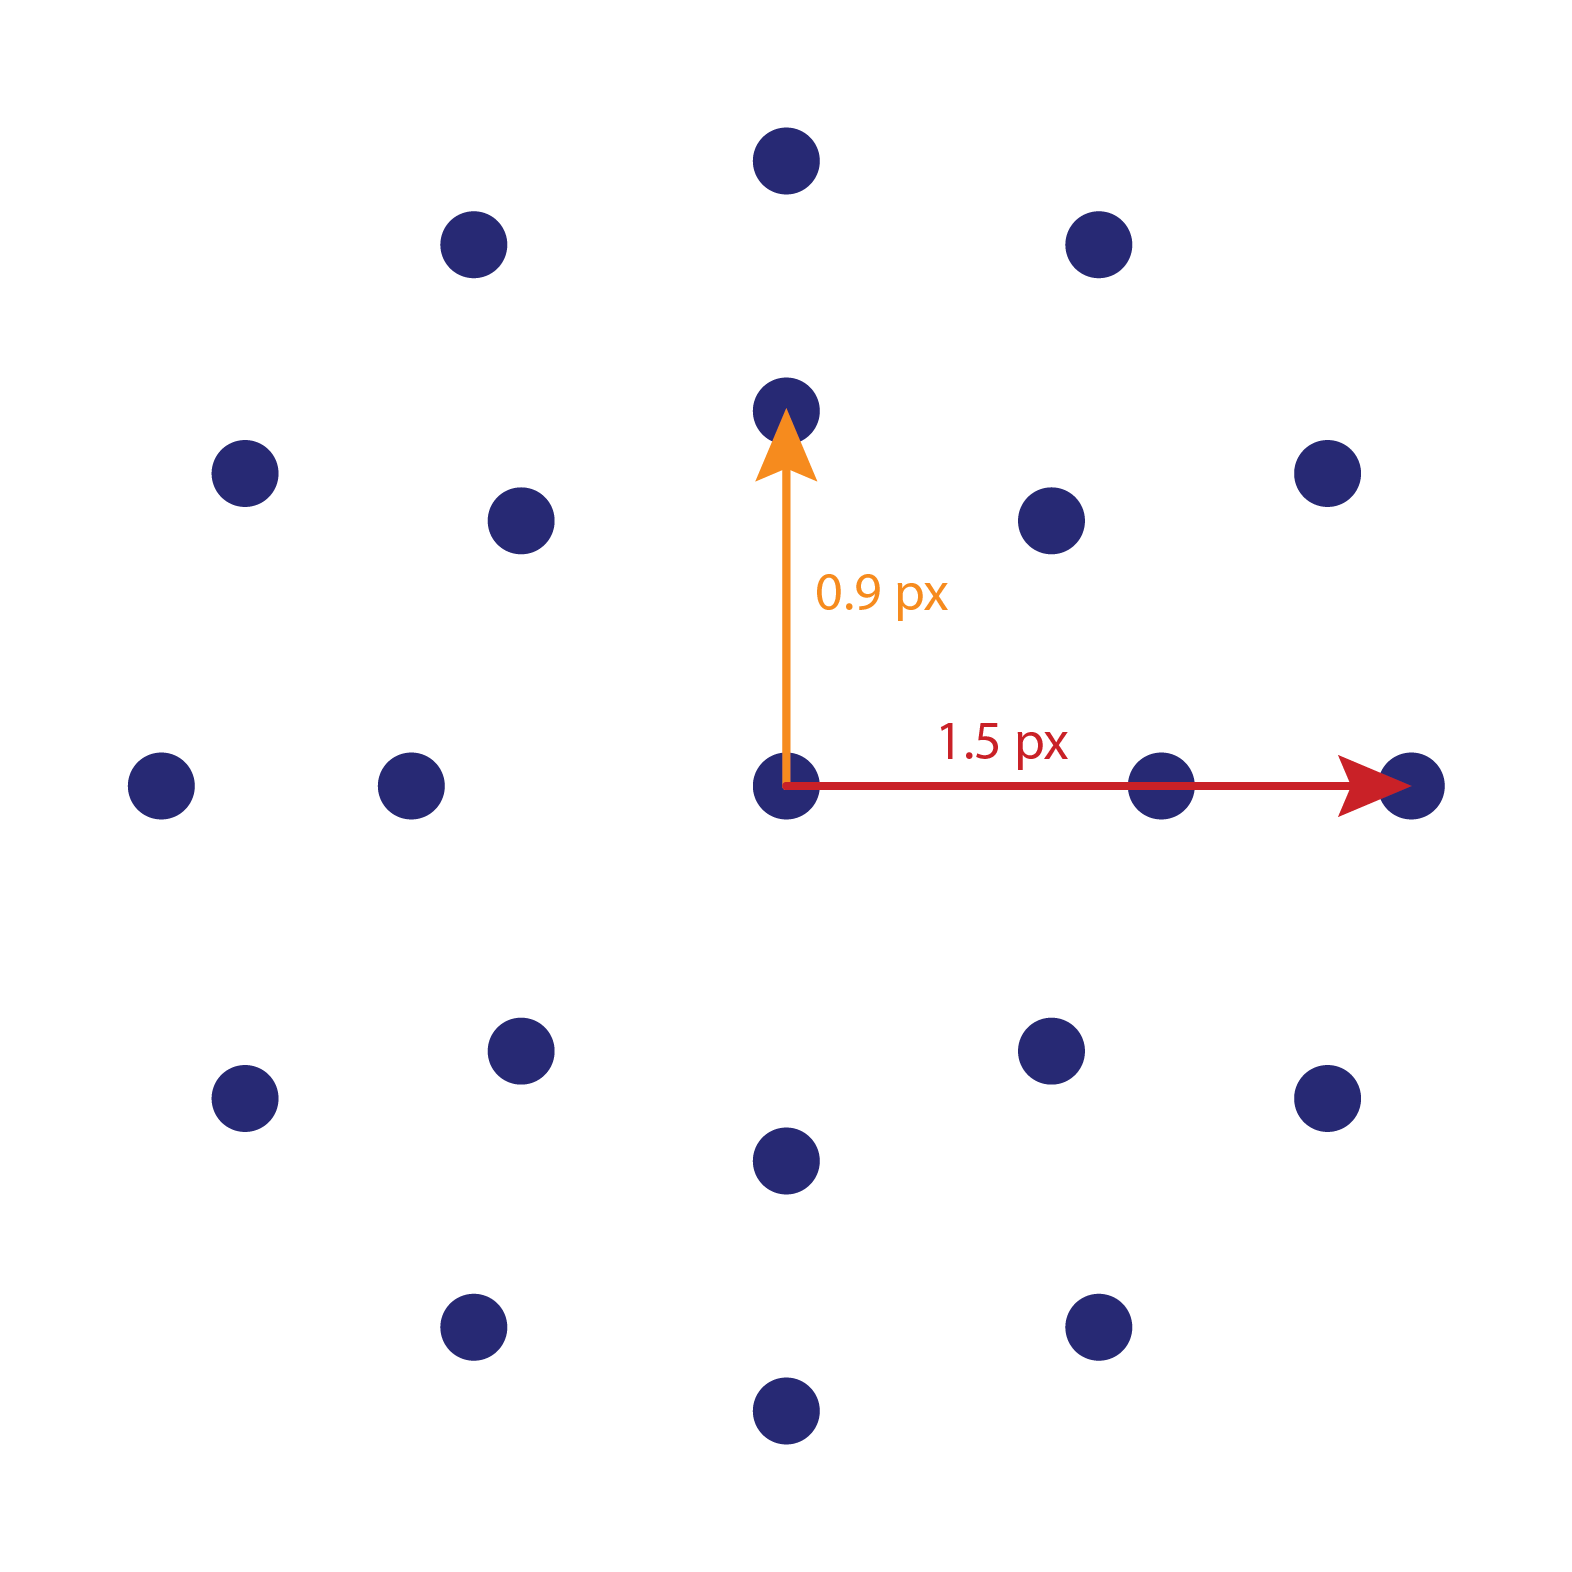
\includegraphics[width=\textwidth-6cm]{images/methode/physics-actionspace.png}
  \caption{Action-Space in der physikalischen Umgebung (eigene Abbildung)}
  \label{fig:physics-actionspace}
\end{figure}


Mit dem gewählten Beschleunigungsvektor $\vec{a}(t)$ berechnet sich die
Geschwindigkeit im nächsten Step $t+1$ aus dem aktuellen Step $t$ durch folgende
Formel:
\[ \vec{v}(t+1) = \vec{v}(t) + \vec{a}(t) \] Der Betrag der Geschwindigkeit
$\vec{v}(t+1)$ des Agents wird in jedem Step, unabhängig von der gewählten
Action, um $0.3$ Pixel pro Step verringert. Das simuliert eine Reibungskraft,
die auf den Agent einwirkt.


Die Veränderungen in der Umgebung erfordern Anpassungen im neuronalen Netz
(siehe \doubleref{sub:t_ml_nn}). Ohne diese Anpassungen kann die KI den
akkumulierten Reward nicht maximieren. Das Problem ist, dass die aktuelle
Geschwindigkeit des Agents kein Teil der Observation ist (siehe
\doubleref{sub:t_rl_func}). Der Agent berücksichtigt deswegen seine
Geschwindigkeit nicht in seinen Entscheidungen. Die Lösung dieses Problems
bietet eine Verschiebung des Local image Patches (siehe \doubleref{sub:t_ver_dood}).
Im Grundprogramm entspricht der Mittelpunkt des Local image Patches genau der
Position des Agents. Neu befindet sich der Mittelpunkt dort, wo sich der Agent
laut seiner aktuellen Geschwindigkeit im nächsten Step befinden wird. Durch
diese Verschiebung des Local image Patches erhält der Agent Informationen über
seine Geschwindigkeit, ohne dessen numerischen Wert zu kennen. Wie im
Grundprogramm gibt der Local image Patch den gesamten Bereich an, in dem sich
der Agent im nächsten Step befinden kann. Die tatsächliche neue Position des
Agents wird durch die Action seiner Wahl bestimmt. Die Grösse des Local image
Patches schrumpft von $7\times7$ Pixeln auf $5\times5$ Pixel, da alle möglichen
Positionen des Agents nach einem Step auf einem $5\times5$ Feld Platz haben
(siehe \autoref{fig:patch-move}). 

%bild local patch verschiebung
\begin{figure}[!ht]
  \centering
  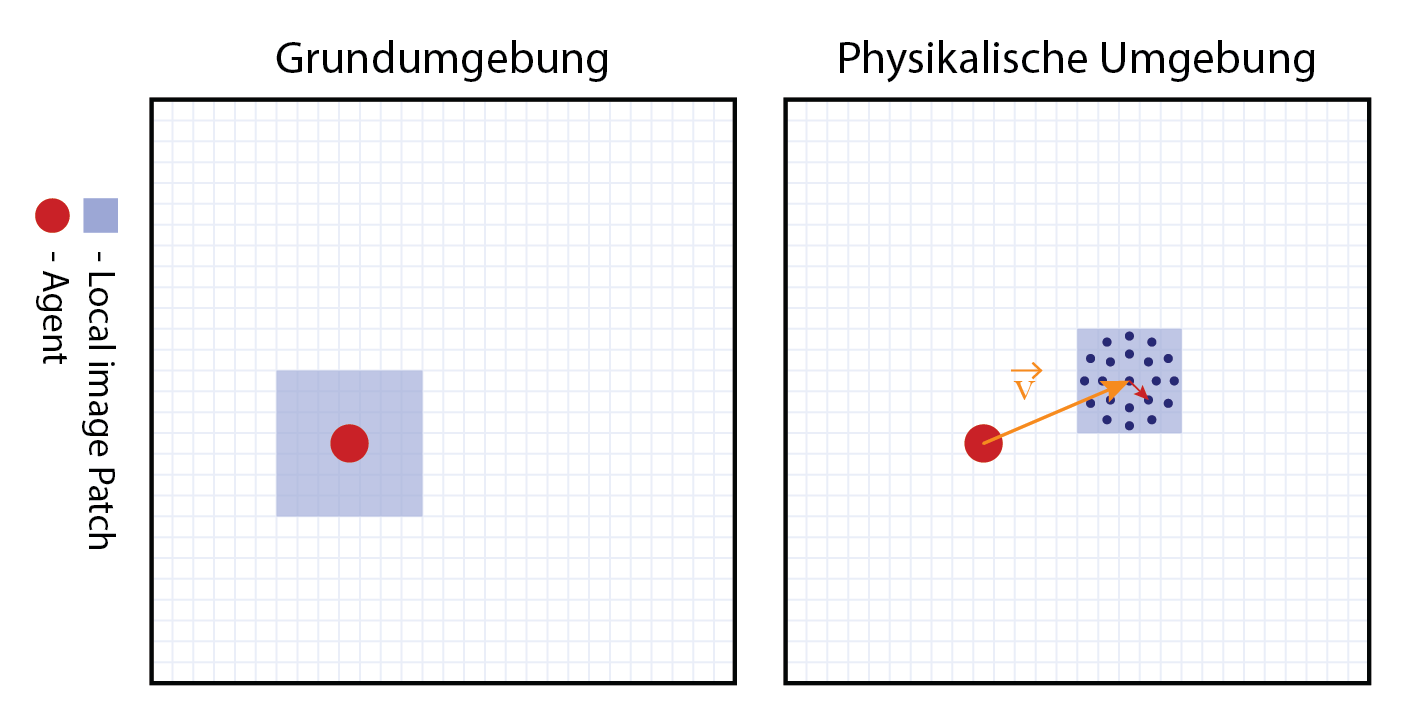
\includegraphics[width=\textwidth]{images/methode/patch-move.png}
  \caption{Angabe der Geschwindigkeit durch eine Verschiebung des Local image Patches (eigene Abbildung)}
  \label{fig:patch-move}
\end{figure}


Ein weiteres Problem ist, dass der Agent sich durch seine Geschwindigkeit aus
den vorgegebenen Grenzen der Zeichenfläche begeben kann. Im Grundprogramm  
(siehe \doubleref{sub:m_grund_dood}) kann der Agent Actions, die ihn in eine
unzulässige Position bewegen würden, nicht auswählen. Wenn allerdings in der
phyiskalischen Umgebung die Geschwindigkeit des Agents zu hoch ist, kann dieser
keine Actions mehr wählen, die ihn innerhalb der Grenzen der Zeichenflächen
halten würden. Als Lösung wird diesen Fällen die Geschwindigkeit des Agents auf den
Nullvektor zurückgesetzt und die Reward Function löst einen negativen Reward von
$-0.05$ aus. Der negative Reward soll die Häufigkeit dieser Vorfälle vermindern.


\section{Auswertung}\label{chap:m_auswert}
Die Auswertung der Daten über die Leistung der künstlichen Intelligenz liefert
das Resultat der Methode. Die Auswertung berechnet den Zahlenwert der
definierten Kriterien (siehe \doubleref{chap:m_eval}) für verschiedene Variationen
der KI.

Die Variationen werden auf ihre Leistung für drei verschiedene Datensets
geprüft. Die drei Datensets beinhalten verschiedene Arten von handgemachten
Strichbildern (siehe \autoref{tab:models}). Im Falle des QuickDraw datensets
wird die KI allerdings nur auf das Nachzeichnen von zehn Motiven überprüft. Die
zehn Motive sind: `Amboss', `Apfel', `Besen', `Eimer', `Bulldozer', `Uhr',
`Wolke', `Computer', `Auge' und `Blume' (siehe
\autoref{fig:quickdraw-examples}). Die Bilder in den drei Datensets sind gleich
verarbeitet wie die Trainingsdaten (siehe \doubleref{sub:m_grund_data}). 

%Bild images dataset
\begin{figure}[!ht]
  \centering
  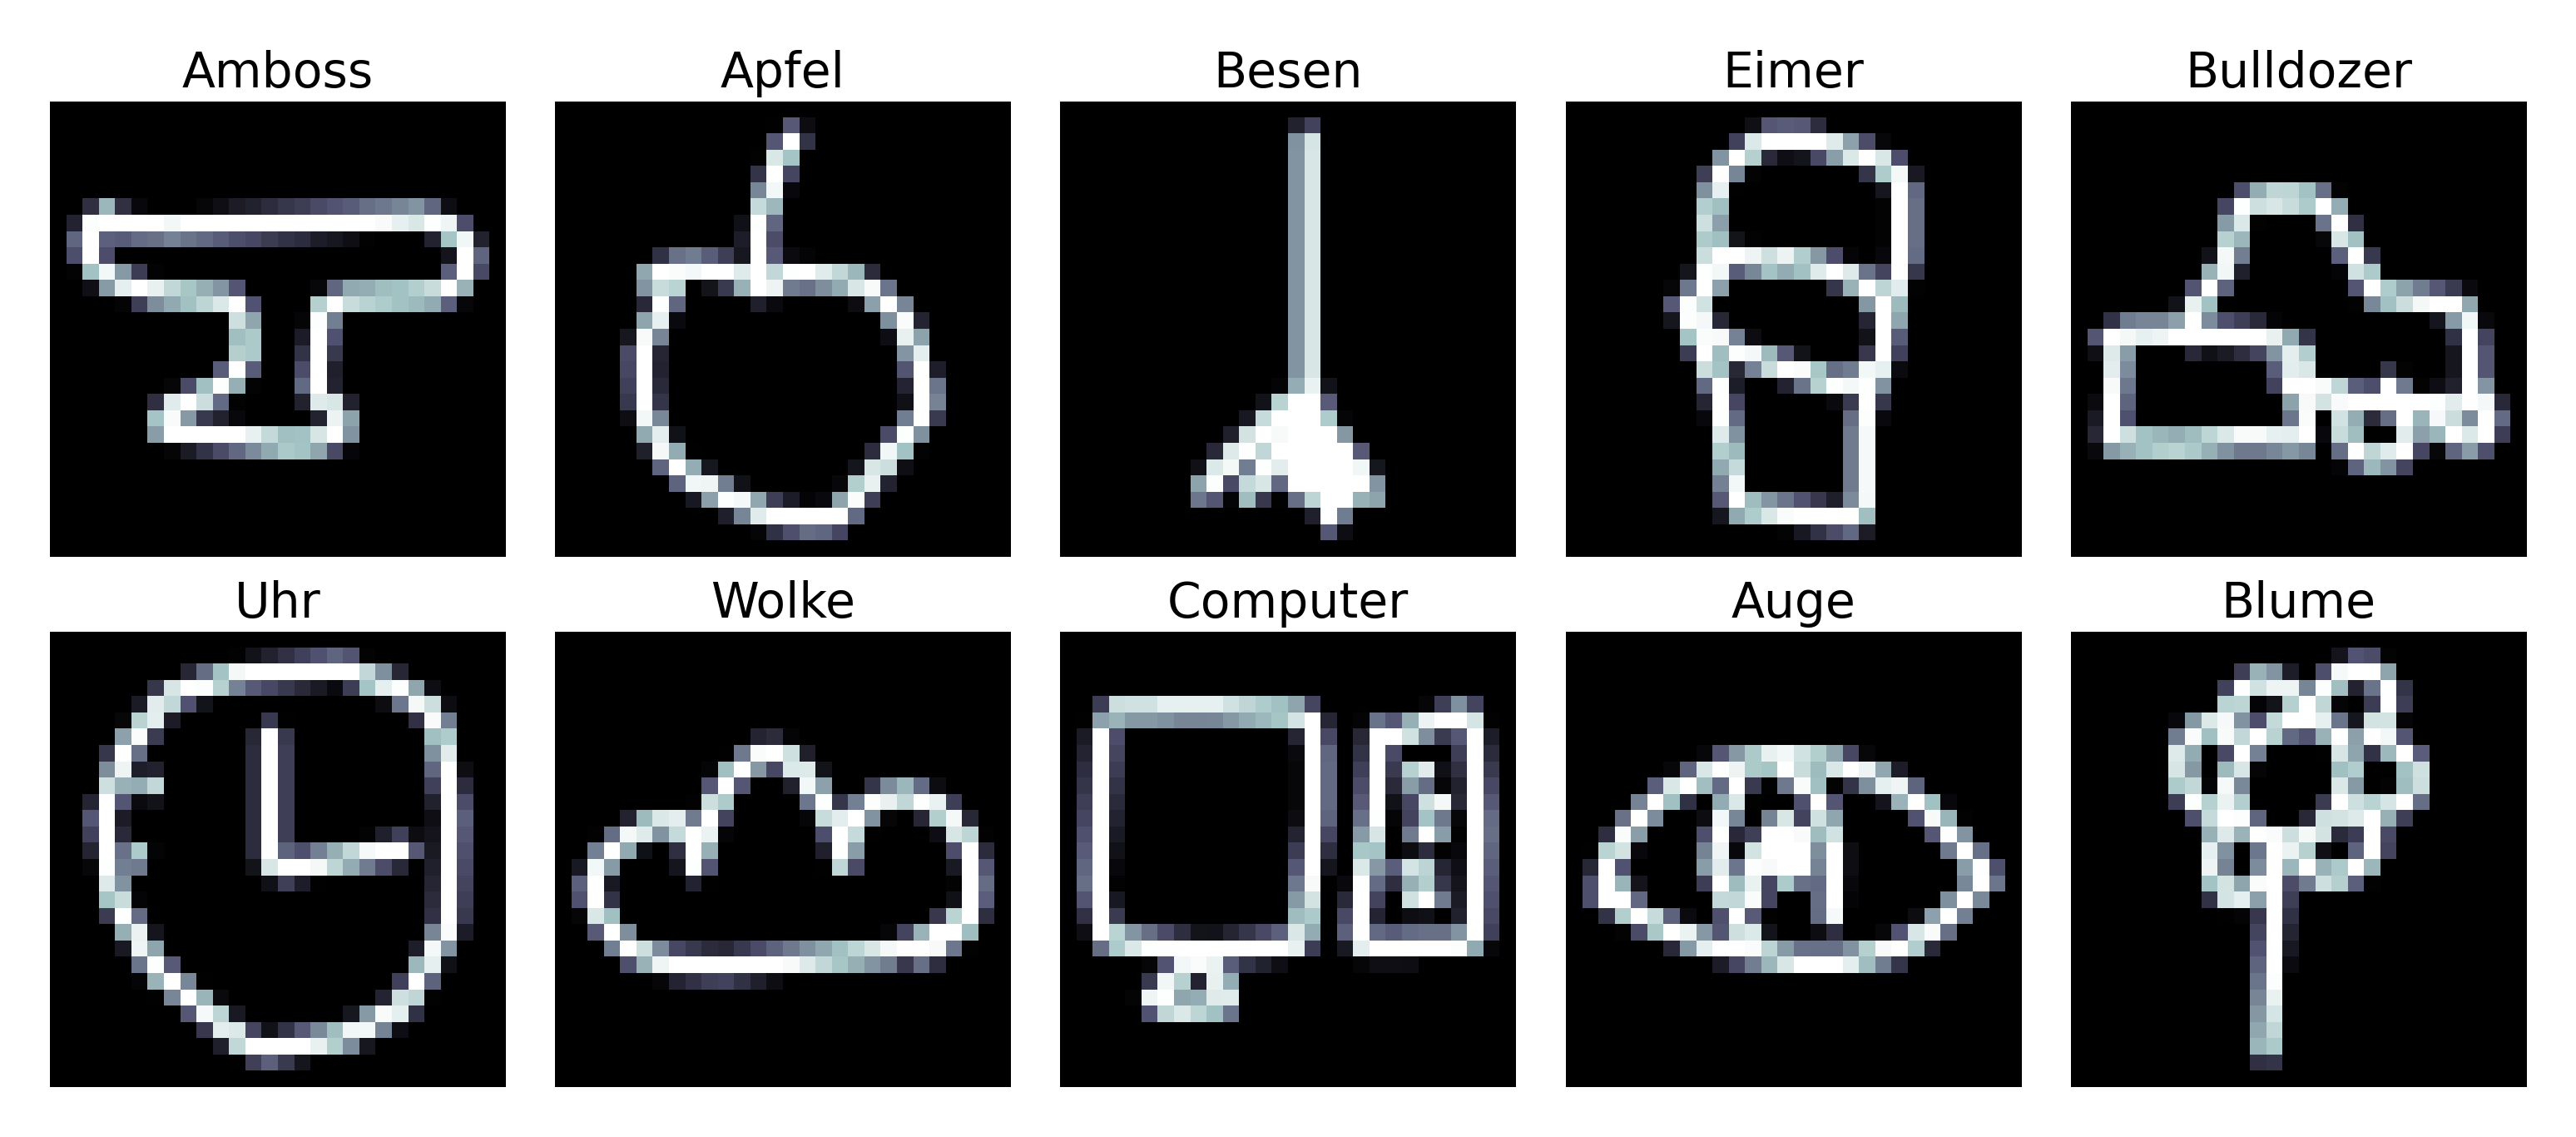
\includegraphics[width=\textwidth]{images/methode/quickdraw-examples.png}
  \caption{Beispiele der verwendeten Motive aus dem QuickDraw Datenset}
  \label{fig:quickdraw-examples}
\end{figure}


Die Variationen (siehe \doubleref{chap:m_var}) der KI umfassen zwei Umgebungen und
drei Reward-Functions (siehe \doubleref{sub:t_rl_func}). Für jede Variation ist zur
Vereinfachung eine Abkürzung definiert.
\begin{itemize}
  \item \doubleref{chap:m_grund} Umgebung: Grund
  \item \doubleref{sub:m_var_phy}: Physik
  \item \doubleref{sub:m_var_base}: Basis
  \item \doubleref{sub:m_var_speed}: Speed
  \item \doubleref{sub:m_var_rec} (von MNIST Ziffern): MNIST
\end{itemize}

Die folgenden Kombinationen an Variationen der künstlichen Intelligenz werden
ausgewertet. Diese Kombinationen stellen einzelne Versionen der KI dar
\begin{itemize}
  \item Grund-Basis
  \item Grund-MNIST
  \item Grund-Speed
  \item Grund-MNIST-Speed 
  \item Physik-Basis
  \item Physik-MNIST
  \item Physik-Speed
  \item Physik-MNIST-Speed
\end{itemize}

\subsection{Testumgebung}\label{sub:m_auswert_test} Die Leistungen der
verschiedenen Variationen der künstlichen Intelligenz werden in einer
Testumgebung (siehe \doubleref{sub:t_ml_func}) ausgewertet. Zwischen der
Trainingsumgebung und der Testumgebung sind drei relevante Unterschiede. Erstens
trainiert die KI in der Testumgebung nicht. Die Testumgebung übernimmt eine
trainierte Version der KI und verändert diese während dem Test nicht. Zweitens
wählt der Agent in keinem Fall mehr eine zufällige Action. Stattdessen wählt er
immer die Action mit dem höchsten Q-Value (gleichbedeutend mit $\epsilon = 0$)
(siehe \doubleref{sub:t_rl_func}). Der Dritte Unterschied liegt in den
Strichbildern, die für die künstliche Intelligenz als Vorlage dienen. Im Test
zeichnet das Computerprogramm $2000$ Bilder aus einem der drei zur Verfügung
stehenden Datensets (siehe \autoref{tab:models}). 

Am Ende jeder Episode (das heisst jeder Zeichnung), wird der Zahlenwert für die
verschiedenen Kriterien (siehe \doubleref{chap:m_eval}) ihrer Definition
entsprechend ausgewertet und gespeichert. Der Durchschnitt aller gespeicherten
Werte eines Kriteriums entspricht der Leistung der getesteten Variation in
diesem Kriterium. Das Kriterium der Erkennbarkeit verwendet zur Auswertung
dasjenige vortrainierte Modell, das auf den selben Daten trainiert ist, die im
Test verwendet werden (siehe \doubleref{sub:m_eval_rec}). Da das Kriterium der
Erkennbarkeit entweder den Wert $0$ oder $1$ hat, ergibt der Durchschnitt aus
allen Werten dieses Kriteriums eine prozentuale Angabe (in Dezimalform) darüber,
in wie vielen Fällen das richtige Motiv erkannt wird.




\chapter{Resultate}\label{chap:r}
Die Resultate bestehen aus drei Tabellen. Jede Tabelle beschreibt die Leistung
der acht Versionen (siehe \doubleref{chap:m_var}), bezogen auf die drei definierten
Kriterien (siehe \doubleref{chap:m_eval}). Die Daten in den Tabellen
stammen aus den Tests der KI (siehe \doubleref{chap:m_auswert})
Der Unterschied in den Tabellen liegt im Datenset, mit denen die Versionen der
KI jeweils getestet sind. 
Eine Sammlung von gezeichneten Strichbildern ergänzt die Resultate. Die
Strichbilder sind dabei jeweils in Paaren angeordnet. Das linke Bild im Paar
zeigt die Vorlage aus dem Datenset und das rechte Bild zeigt die nachgezeichnete
Variante von der KI. Die Zeichnungen, die in der Sammlung
vertreten sind, sind zufällig ausgewählt aus dem Test der jeweiligen Version der
KI. Die Bilder haben einen Farbverlauf, der den zeitliche
Verlauf des Zeichnens dargestellt. Die Helligkeit eines Striches ist
proportional zu dem Step, in dem dieser gezeichnet wurde. Das bedeutet, dass
dunklere Striche früher gezeichnet werden als hellere Striche. Bewegungen des
Agents, in denen dieser nicht zeichnet, sind in den Bildern nicht erkennbar.

\newpage
\section{Tabellen}\label{chap:r_tab}
\begin{table}[!ht]
    \centering
    \caption{Testen auf MNIST Datenset | 2000 Tests}\label{tab:MNIST}
    \begin{tabular}{|l|l|l|l|}
        \hline
            ~ & Übereinstimmung \% & Erkennbarkeit \% & Geschwindigkeit \\ \hline
            Grund-Basis & 86.5 & 86.6 & 24.5 \\ \hline
            Grund-MNIST & 66.8 & 64.3 & 51.2 \\ \hline
            Grund-Speed & 86.2 & 86.6 & 25.5 \\ \hline
            Grund-MNIST-Speed & 61.4 & 55.1 & 56.8 \\ \hline
            Physik-Basis & 56.4 & 46.4 & 62.5 \\ \hline
            Physik-MNIST & 38.4 & 35.7 & 63.9 \\ \hline
            Physik-Speed & 63.0 & 58.2 & 61.2 \\ \hline
            Physik-MNIST-Speed & 29.2 & 27.3 & 63.7 \\ \hline
        \end{tabular}
\end{table}

\begin{table}[!ht]
    \centering
    \caption{Testen auf EMNIST Datenset | 2000 Tests}\label{tab:EMNIST}
    \begin{tabular}{|l|l|l|l|}
    \hline
        ~ & Übereinstimmung \% & Erkennbarkeit \% & Geschwindigkeit \\ \hline
        Grund-Basis & 86.8 & 74.5 & 38.2 \\ \hline
        Grund-MNIST & 65.2 & 45.0 & 57.4 \\ \hline
        Grund-Speed & 87.8 & 77.0 & 37.7 \\ \hline
        Grund-MNIST-Speed & 62.2 & 40.0 & 60.9 \\ \hline
        Physik-Basis & 57.6 & 32.4 & 63.5 \\ \hline
        Physik-MNIST & 43.3 & 23.6 & 63.9 \\ \hline
        Physik-Speed & 56.3 & 35.0 & 63.6 \\ \hline
        Physik-MNIST-Speed & 30.2 & 13.9 & 64.0 \\ \hline
    \end{tabular}
\end{table}

\begin{table}[!ht]
    \centering
    \caption{Testen auf QuickDraw-Datenset | 2000 Tests}\label{tab:Quickdraw}
    \begin{tabular}{|l|l|l|l|}
    \hline
        ~ & Übereinstimmung \% & Erkennbarkeit \% & Geschwindigkeit \\ \hline
        Grund-Basis & 79.1 & 80.5 & 39.1 \\ \hline
        Grund-MNIST & 57.3 & 62.5 & 59.9 \\ \hline
        Grund-Speed & 79.5 & 82.2 & 40.0 \\ \hline
        Grund-MNIST-Speed & 54.9 & 58.9 & 62.5 \\ \hline
        Physik-Basis & 48.1 & 55.7 & 63.8 \\ \hline
        Physik-MNIST & 30.5 & 38.9 & 64.0 \\ \hline
        Physik-Speed & 50.0 & 58.3 & 63.6 \\ \hline
        Physik-MNIST-Speed & 22.4 & 31.1 & 64.0 \\ \hline
    \end{tabular}
\end{table}

\newpage

\section{Bildersammlung}\label{chap:r_bild}
\begin{figure}[!ht]
    \centering
    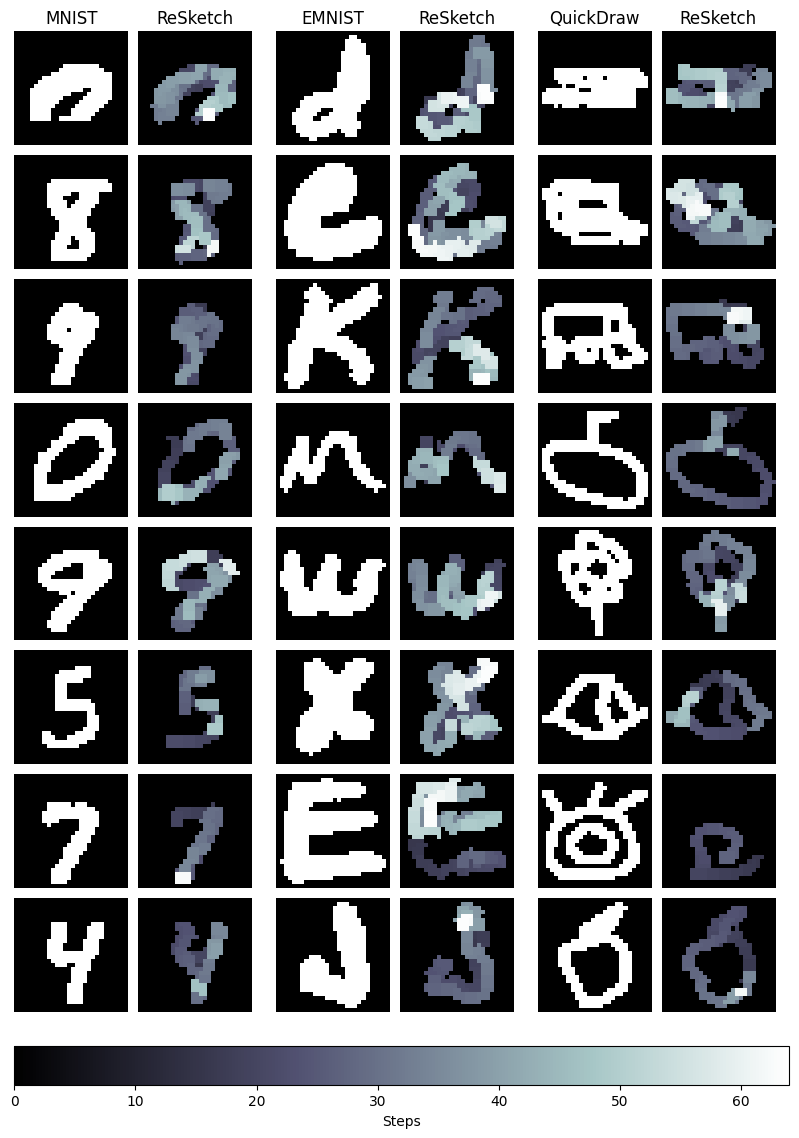
\includegraphics[width=\textwidth]{images/resultate/base-base.png}
    \caption{Grund-Basis}\label{fig:Grund-Basis}
\end{figure}

\newpage
\begin{figure}[!ht]
    \centering
    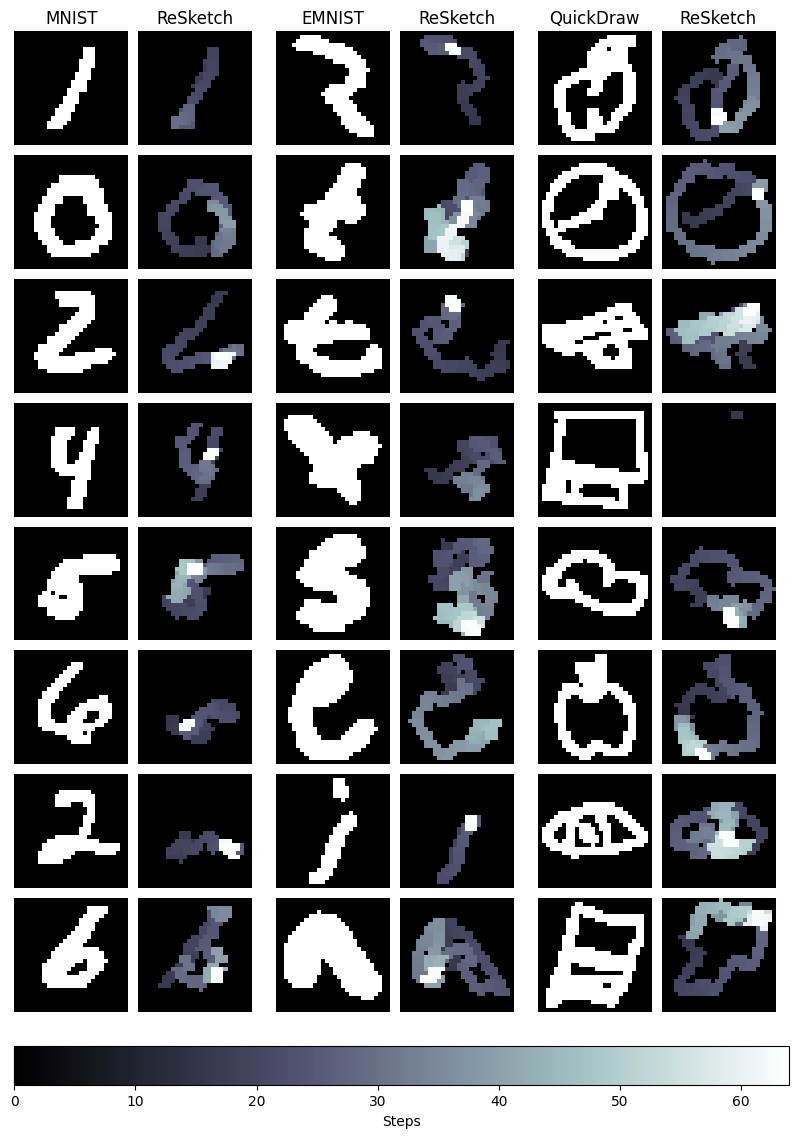
\includegraphics[width=\textwidth]{images/resultate/base-mnist.png}
    \caption{Grund-MNIST}\label{fig:Grund-MNIST}
\end{figure}

% \begin{figure}[!ht]
%     \centering
%     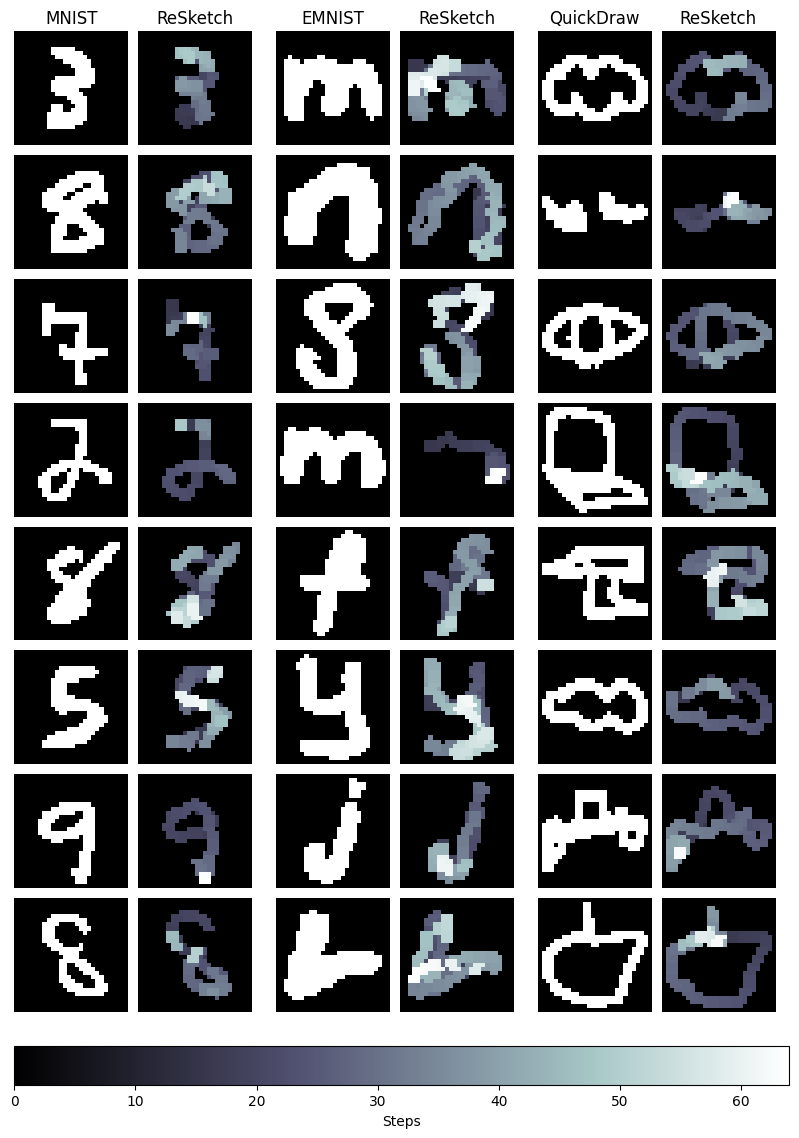
\includegraphics[width=\textwidth]{images/resultate/base-speed.png}
%     \caption{Grund-Speed}
%     \label{fig:Grund-Speed}
% \end{figure}

\begin{figure}[!ht]
    \centering
    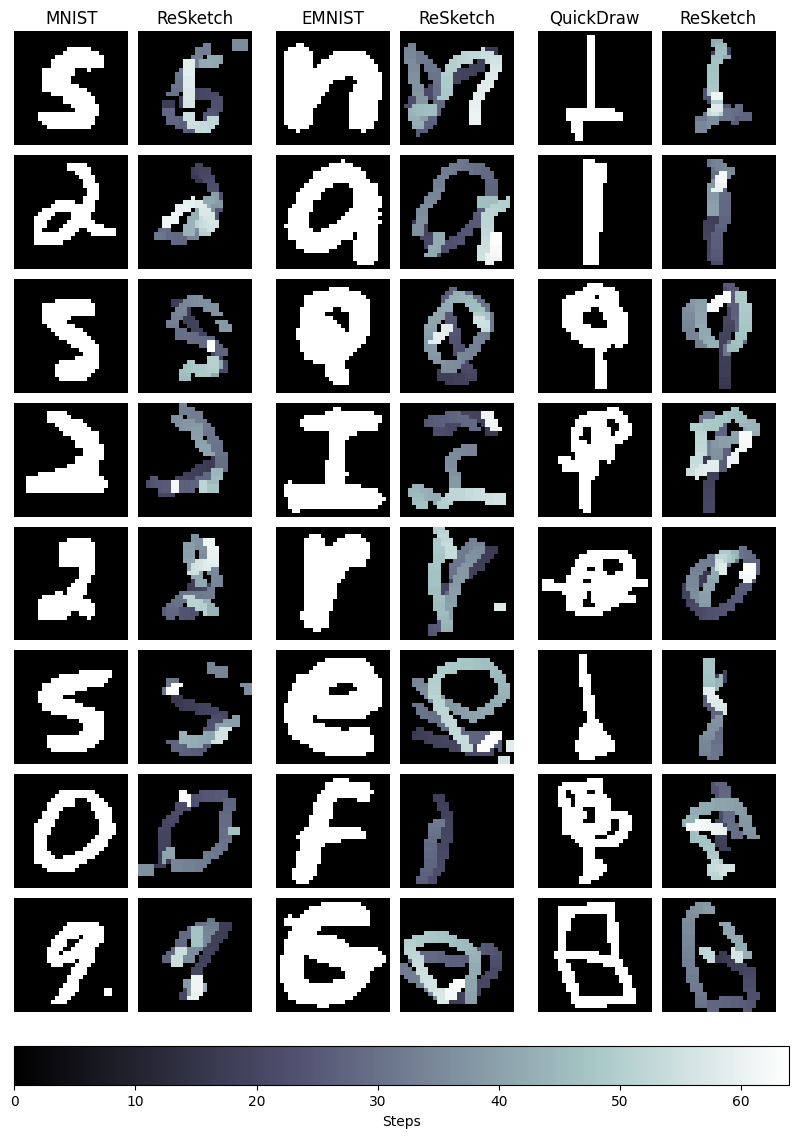
\includegraphics[width=\textwidth]{images/resultate/physics-base.png}
    \caption{Physik-Basis}\label{fig:Physik-Basis}
\end{figure}

\begin{figure}[!ht]
    \centering
    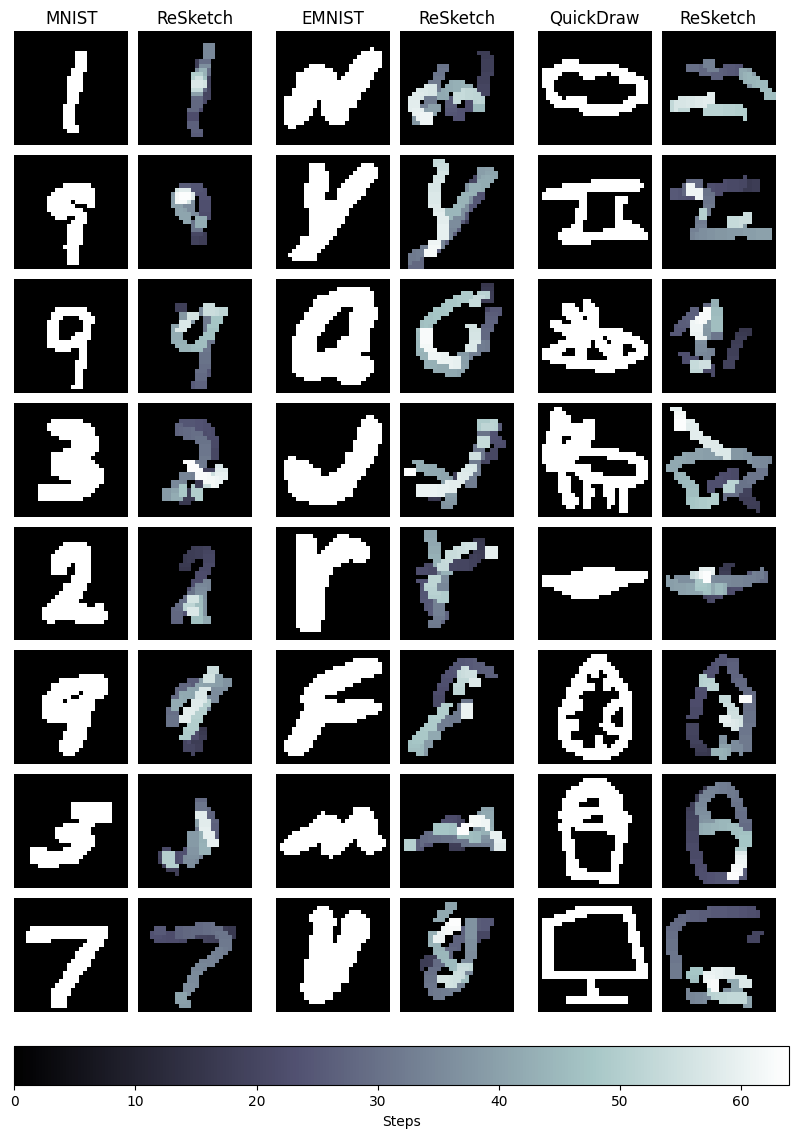
\includegraphics[width=\textwidth]{images/resultate/physics-speed.png}
    \caption{Physik-Speed}\label{fig:Physik-Speed}
\end{figure}

\chapter{Diskussion}\label{chap:d}
Die Diskussion analyisiert die Resultate der Methode (siehe \nameref{chap:m}),
um daraus eine Antwort auf die Fragestellung zu bilden. Zu diesem Zweck werden
einige allgemeine Feststellungen getroffen  und die Unterfragen beantworten
(siehe \ref{chap:d_frage} \nameref{chap:d_frage}). Im zweiten Teil der Diskussion folgt ein Fazit,
ein Ausblick (siehe \nameref{chap:d_faz-aus}), und eine Selbstreflexion (siehe
\nameref{chap:d_reflex}). Dabei verschiebt sich der Fokus von der Fragestellung
weg und auf eine allgemeinere Betrachtung der Arbeit.


\section{Fragestellung und Unterfragen}\label{chap:d_frage}
Die Fragestellung und die Unterfragen decken nicht alle Erkenntnisse aus den
Resultaten ab. Einige allgemeine Feststellungen geben Einblick, wie die
Resultate (siehe \nameref{chap:r}) zu verstehen sind. 

Die Grund-Basis Version und die Grund-Speed Version (siehe
\nameref{chap:m_auswert}) erreichen in allen Kriterien für alle Datensets die
beste Leistung. Die Resultate zwischen den Versionen sind dabei fast
ununterscheidbar. Vor allem im Kriterium der Geschwindigkeit (siehe
\nameref{sub:m_eval_speed}) zeigt die Speed Variation keine Verbesserung. Unter
den Versionen, die auf der physikalischen Umgebung basieren, erreichen Ebenfalls
die Physik-Basis und die Phyisk-Speed Versionen die beste Leistung. Die
Grund-MNIST Version und die Physik-MNIST Version sind in allen Kriterien
schlechter als die Basis und Speed Versionen. Auch im Kriterium der
Erkennbarkeit (siehe \nameref{sub:m_eval_rec}) bringt die Variation keinen
Vorteil. Die Physik-MNIST-Speed Version erbringt die schlechteste Leistung. Eine
Erklärung dafür ist, dass diese Version eine Kombination von allen Variationen
(siehe \nameref{chap:m_var}) ist und somit von der besten Version, der
Grund-Basis Version am stärksten abweicht.

Die Bildersammlung (siehe \nameref{chap:r_bild}) zeigt, dass die KI in vielen
Fällen präzise der Linie folgt und selten willkürliche Sprünge begeht. Das ist
interessant, weil der KI nie explizit mitgeteilt wird, wie genau sie zeichnen
sollte.


\subsection{Beantwortung der Unterfragen}\label{sub:d_frage_unter}
Insgesamt sechs Unterfragen werden beantwortet (siehe \nameref{chap:einleit}).
Diese Unterfragen weiten die Fragestellung aus und tragen zu der
schlussendlichen Antwort auf die Fragestellung bei. Die Antworten beruhen auf
den Resultaten, aber auch auf Erkenntnissen aus der Methode (siehe
\nameref{chap:m}) selbst.

\subsubsection*{Wie kann die Architektur einer KI aussehen, die das Nachzeichnen erlernt?}\label{subsub:d_frage_unter_1}
Unter der Annahme, dass die KI dieser Arbeit das Nachzeichnen erlernt, (siehe
\nameref{sub:d_frage_frag}), kann die Architektur genau so aussehen, wie sie in
dieser Arbeit beschrieben ist (siehe \nameref{sub:m_grund_dood}).

\subsubsection*{Wie lässt sich die Leistung der KI in dieser Aufgabe beurteilen?}\label{subsub:d_frage_unter_2}
Die Leistung der KI lässt sich durch die definierten Kriterien (siehe
\nameref{chap:m_eval}) beurteilen. Das Kriterium Die Übereinstimmung ist ein
objektiver und Absoluter Wert, und somit das Aussagekräftigste Kriterium.
Ausserdem ist der maximale Wert des Kriteriums, unabhängig vom gezeichneten
Bild, gleich $1$. Dadurch ist das Kriterium geeignet für Vergleiche zwischen
Versionen der KI.

die Kriterien der Erkennbarkeit und der Geschwindigkeit sind an subjektive
Annahmen gebunden. Zum Beispiel wird für das Kriterium der Geschwindigkeit ein
subjektiver Punkt der Fertigstellung definiert (siehe
\nameref{sub:m_eval_speed}). Dadurch sinkt ihre Aussagekraft. Allerdings
verändern sich die Annahmen nicht und die Kriterien sind in jedem Fall durch
einen Zahlenwert repräsentiert. Somit eignen sich auch diese Kriterien für
Vergleiche zwischen Versionen der KI. Aus der Annahme heraus, dass für Menschen
beim Nachzeichnen Erkennbarkeit wichtiger als absolute Genauigkeit ist, ergibt
sich das Kriterium der Erkennbarkeit als besonders wichtiges. Aus diesem Grund
ist das Kriterium in der Fragestellung (siehe \nameref{sub:d_frage_frag})
vermerkt.


\subsubsection*{Wie lässt sich die Leistung der KI verbessern?}\label{subsub:d_frage_unter_3}
Bezogen auf die definierten Kriterien erreicht die Grundversion Werte, die durch
die implementierten Variationen nicht oder nur marginal verbessert werden. Die
Variationen der KI sind somit insgesamt ein gescheiterter Versuch der
Verbesserung der Leistung. Die Grundversion erfuhr allerdings in dessen
Entwicklung signifikante Verbesserungen. Die grössten Verbesserungen stammen aus
der Optimierung der Hyperparamter durch den Baysian Optimization Algorithmus
(siehe \nameref{sub:m_grund_data}). Zum Beispiel hat die Grösse des Replay
Buffers einen erheblichen Effekt auf die Leistung.

\subsubsection*{Welche Einflüsse haben Physiksimulationen auf die Leistung der KI?}\label{subsub:d_frage_unter_4}
Bezogen auf die definierten Kriterien verschlechtert sich die Leistung der KI.
Alle Versionen, die auf der Grundumgebung basieren, erzielen höhere Werte als
die gleichen Versionen basierend auf der phyiskalischen Umgebung (siehe
\nameref{sub:m_var_phy}). Die physikalische Umgebung hat zum Ziel, die
Bewegungen der KI realistischer zu gestalten. In diesem Bereich kann der
Einfluss nicht objektiv bestimmt werden. Aus Beobachtungen der Bilder, welche in
der physikalischen Umgebung gezeichnet sind (siehe \nameref{chap:r_bild}), gehen
ebenfalls keine Erkenntnisse in diesem Bereich hervor. Die Bilder unterscheiden
sich kaum von denjenigen aus der Grundumgebung.

\subsubsection*{Wie ändert sich die Leistung der KI bei Strichbildern, die sich von den Trainingsdaten unterscheidenn}\label{subsub:d_frage_unter_5}
In allen acht Versionen bleibt die Leistung der KI zwischen den drei Datensets
(siehe \autoref{tab:datasets}) vergleichbar. Die Tabellen {...} und {...} Zeigen
die Leistung der Grund-Basis Version und der Physik-Basis Version in den drei
definierten Kriterien, getestet auf die drei Datensets. Der Wert der
Übereinstimmung zwischen dem MNIST Datenset und dem EMNIST Datenset ist beinahe
identisch. Für beide Versionen ist der Wert der Übereinstimmung für das
QuickDraw Datenset niedriger. Insgesamt ist die KI in diesem Kriterium jedoch
kaum Beeinflusst durch die Wahl des Datensets. Die Analyse der anderen zwei
Kriterien führt zu einer ähnlichen Schlussfolgerung. Interessant ist, dass vor
allem die Grund-Basis Version eine viel höhere Geschwindigkeit im Zeichnen von
MNIST Zahlen hat, als im Zeichnen von EMNIST Buchstaben. Obwohl die Formen zu
grossem Teil ähnlich sind, scheint die KI durch das spezifische Training auf
MNIST Ziffern eine höhere Geschwindigkeit zu entwickeln. 

%todo neue Tabellen

\subsubsection*{Inwiefern lässt sich das Zeichnen der KI mit menschlichem Zeichnen vergleichen?}\label{subsub:d_frage_unter_6}
Die Antwort auf diese Frage leitet sich nicht aus den objektiven Resultaten ab,
sondern basiert auf subjektiven Beobachtungen. Die Bewegungen in der
Physik-Version der künstlichen Intelligenz basieren grundsätzlich auf den selben
Gesetzen wie die Bewegungen in der echten Welt. Allerdings sind die Bewegungen
stark vereinfacht im Vergleich zu menschlichen Bewegungen Ausserdem ist für die
künstliche Intelligenz der Druck des Stiftes nicht veränderbar. Zumindest
Konzeptuell aber nähert die künstliche Intelligenz menschliches Zeichnen,
bezogen auf die physischen Einschränkungen, an. Einige menschliche Gewohnheiten
sind bei der künstlichen Intelligenz allerdings nicht beobachtbar. Zum Beispiel
beginnt die künstliche Intelligenz beim Zeichnen von Ziffern an zufälligen
Orten, während Menschen in der Regel für jede Ziffer an der selben Stelle
ansetzen einer Ziffer immer an der selben Stelle


\subsection{Beantwortung der Fragestellung}\label{sub:d_frage_frag}
Die Fragestellung lautet: in wiefern kann eine künstliche Intelligenz lernen,
Strichbilder auf eine physische Weise nachzuzeichnen, sodass diese durch ein
automatisches System erkannt werden? (siehe \nameref{chap:einleit}) Diese Frage
hat mehrere Aspekte, die teilweise bereits durch die Unterfragen (siehe
\nameref{sub:d_frage_unter}) erfasst werden. Für die schlussendliche Antwort
folgt eine genauere Ausführung der Aspekte.

Die KI zeichnet durch Physiksimulationen und durch allgemeine Einschränkungen
der Bewegungsfreiheit auf eine annähernd physische Weise. Das Zeichnen ist nur
annähernd physisch, da alle Bewegungen simuliert und in keiner phyischen
Umgebung umgesetzt sind. Ausserdem sind die Simulationen nicht vollkommen
realitätsgetreu (siehe \ref{sub:d_frage_unter} \nameref{subsub:d_frage_unter_4})

Die künstliche intelligenz erlernt das Nachzeichnen bezogen auf die Kriterien,
nach denen es definiert ist, erfolgreich. Dafür sprechen die Werte der besten
Versionen für das Nachzeichnen von Ziffern, die teilweise an den Höchstwert
grenzen (siehe \nameref{chap:d_frage}). Die hohen Werte im Kriterium der
Erkennbarkeit bestätigen ausserdem, dass die Zeichnungen der KI in den meisten
Fällen von einem automatischen System erkannt werden.

Laut der Fragestellung soll die KI das Nachzeichnen von Strichbildern erlernen.
Damit ist implizit das Nachzeichnen von allen möglichen Arten von Strichbildern
gemeint. Die Leistung der KI kann nicht auf alle möglichen Strichbilder
überprüft werden, aber der Test mit drei verschiedenen Datensets ergibt
vielversprechende Resultate (siehe \nameref{chap:r_tab}). Die KI erlernt
erfolgreich das Nachzeichnen von Ziffern, Kleinbuchstaben und zehn zufälligen
Motiven aus dem QuickDraw Datenset. Durch die Vielfalt im QuickDraw Datenset
kann die Annahme getroffen werden, dass die KI zumindest einen grossen Teil an
Strichbildern nachzeichnen kann. 

Die zusammenfassende Antwort auf die Frage lautet somit: Eine künstliche
Intelligenz kann das Nachzeichnen von Strichbildern auf annähernd physiche Weise
in dem Sinne lernen, dass die fertige Zeichnung von einem automatischen System
grösstenteils erkannt wird, Die Übereinstimmung zwischen der Vorlage und der
Zeichnung gross ist und die Zeichnung nicht viel Zeit in Anspruch nimmt.

Diese Antwort bezieht sich auf die genau Frage, wie sie in der Einleitung steht.
Der nächste Abschnitt beurteilt die Frage durch die Erkenntnisse aus dieser
Arbeit und geht auf mögliche Erweiterungen ein.


\section{Fazit und Ausblick}\label{chap:d_faz-aus}
Die Resultate erlauben eine positive Antwort auf die Fragestellung. Diese
Antwort setzt allerdings einige Annahmen vorraus, die weiter diskutiert werden
können. Die grösste Annahme bezieht sich auf die Definition des Nachzeichnens.
Diese Arbeit definiert Nachzeichnen durch drei Kriterien und durch physische
Rahmenbedingungen. Die Kriterien sind für eine künstliche Intelligenz sinnvoll
gewählt (siehe \nameref{subsub:d_frage_unter_2}), Allerdings wären auch ander
Kriterien möglich. Nachzeichnen ist eine menschliche Tätigkeit. Dieser
Menschliche Aspekt ist in den definierten Kriterien nicht enthalten.

Die physichen Rahmenbedingungen unterscheiden sich von denjenigen, die ein
Mensch erfährt. Das kommt daher, dass die phyischen Rahmenbedingungen für die KI
lediglich simuliert sind. Das verunmöglicht eine umfassende Antwort auf die
Frage, ob die künstliche Intelligenz auf eine physische Weise zeichnet. Dieses
Problem könnte mit einem Roboter gelöst werden, der die künstliche Intelligenz
in eine reale, phyische Umgebung überführt. Der Roboter könnte somit
verschiedenste Strichbilder auf einem echten Stück Papier, und somit
zwangsläufig auf physische Weise nachzeichnen. Aktuell sind die Bewegungen der
künstlichen Intelligenz in gewissen Belangen eingeschränkt. So ist
beispielsweise die Druckstärke nicht variierbar. Ausserdem zeichnet die
künstliche Intelligenz vorwiegend kleine Strichbilder. Experimente mit grösseren
Konstrukten, wie ganze Wörter, wären eine mögliche Erweiterung. 

Alles in allem sind eine Vielzahl an denkbaren Fragen und Ideen möglich, die auf
ReSketch, der künstlichen Intelligenz hinter dieser Arbeit, basieren.


\section{Selbstreflexion}\label{chap:d_reflex} Die Selbstreflexion gibt genauere
Einblicke in die Vorangehensweise hinter dieser Arbeit. Diese Dokumentation ist
grundsätzlich eine Zusammenfassung der wichtigsten Ereignisse. Viele Aspekte,
wie auch die Arbeitsweise bleiben verschwiegen. Die selbstreflexion geht näher
auf drei wichitige Aspekte ein, die in der zusammengefassten Dokumentation nicht
genug betont sind.

Die Dokumentation ist mit Latex und spezifischer der ETH Thesis Formatvorlage
\cite{noauthor_cadmo_2014} formatiert. Ein Grossteil der Abbildungen stammt von den Autoren
und ist in Adobe Illustrater oder der Python Library Matplotlib erstellt

\subsection{Optimierung der KI}\label{sub:d_reflex_opti} Insgesamt sind acht
Versionen der KI präsentiert. Im Verlaufe des Projektes gab es viele weitere
Versuche, die Leistung der künstlichen Intelligenz zu verbessern. Diese Versuche
führten allerdings häufig dazu, dass die KI den akkumulierten Reward (siehe
\nameref{sub:t_rl_func}) nicht mehr maximieren konnte. In der Dokumentation sind
deswegen nur diejenigen Versuche vermerkt, die tatsächlich funktionieren. Das
Problem hinter den versuchten Variation liegt darin, dass die Ursache hinter
ihrem Scheitern oder ihrem Erfolg häufig nicht erkennbar ist. Das macht die
Optimierung der künstlichen Intelligenz allgemein schwierig. 

Die Strategie hinter der Optimierung besteht in den meisten Fällen aus
wiederholtem Ausprobieren mit Anpassungen zwischen jedem Versuch. Hilfsmittel,
wie der Baysian Optimization Algorithmus (siehe \nameref{sub:t_ml_hyper}),
vereinfachen diese Aufgabe massgeblich. Tatsächlich ermöglichte der Baysian
Optimization Algorithmus eine Verbesserung der KI von ungefähr $40-50\%$ mehr im
Kriterium der Übereinstimmung (siehe \nameref{sub:m_eval_proc}). Diese Strategie
der Optimierung ist für einen Computer sehr ressourcenintensiv. In den längsten
Optimierungsarbeiten liefen die beiden Computer, auf denen die Arbeit verrichtet
wurde, zusammen länger als $48$ Stunden.

\subsection{Analyse der künstlichen Intelligenz}\label{sub:d_reflex_analys} Eine
Analyse der künstlichen Intelligenz ist notwendig, um die Fragestellung und die
Unterfragen zu beantworten. Aber auch während der Entwicklung der KI ist eine
stetige Analyse nötig, um dise zu verstehen und zu verbessern.

Die Analyse besteht hauptsächlich darin, die Leistung der künstlichen
Intelligenz zu beurteilen. Das geschieht mittels den Kriterien, die für diesen
Zweck definiert sind (siehe \nameref{chap:m_eval}). Die Kriterien sind dabei so
definiert, dass sie für jede mögliche Variation identisch bleiben. Der
durchnittliche akkumulierte Reward ist beispielsweise absichtlich kein
Kriterium. Der akkumulierte Reward  ist abhängig von der Reward-Function (siehe
\nameref{sub:t_rl_func}) und unterscheidet sich somit zwischen Variationen.
Dieser ist somit nicht für einen Vergleich zwischen Variationen geeignet.

% Abschnitt wäre Streichbar
Einzelne Variationen vergleichbar zu halten, ist ein allgemeines Ziel der
Analyse. Deswegen basieren alle Variationen auf der gleichen Architektur der KI.
Die Funktionalität des Grundprogrammes (siehe \nameref{chap:m_grund}) ist
gründlich getestet. Zum Beispiel sind die Testdaten darauf überprüft, dass sie
keine Datenpunkte aus den Trainingsdaten beinhalten. Diese Tests eliminieren
mögliche Fehlerquellen falls die künstliche Intelligenz unerwartetes Verhalten
aufzeigt.

Eine weitere Form von Analyse stammt aus der Sammlung von Daten über das
Lernverhalten der KI. So wird aus jedem Training ein Graph erstellt, der die
durchschnittliche Leistung der KI in jeder Episode erfasst (siehe
autoref{lernkurve}). Die Leistung ist dabei durch den akkumulierten Reward in
jeder Episode repräsentiert. Wie erwähnt können Versionen der KI nicht anhand
ihres akkumulierten Rewards verglichen werden. Der akkumulierte Reward zeigt
allerdings für einzelne Versionen am präzisesten, in wiefern diese ihren Reward
maximieren können.

%todo bild Lernkurve

\subsection{Verwendung von Git und GitHub}\label{sub:d_reflex_git} Die
Verwendung von Git und Github (siehe \nameref{chap:t_git}) erleichtert die
Arbeit an einem Projekt von diesem Ausmass sehr. Die Programme ermöglichen
einfache Zusammenarbeit am Programmcode und an der Dokumentation. GitHub dient
dabei zusätzlich als Hilfsmitel zur Organisation durch die integrierte Funktion
der Project Boards. Diese Funktion hätte allerdings zu grösserem Ausmass
Verwendung finden können.

Die Funktion der Branches und Commits von Git werden durch die Arbeit hindurch
konsequent verwendet. Dabei wird die Giflow Arbeitsweise, abgesehen von den
Release Branches und den Hotfix Branches, angewendet (siehe
\nameref{sub:t_git_git}) Neben den Feature Branches werden ausserdem
Dokumentation Branches eingeführt, in denen jeweils ein Kapitel der
Dokumentation verfasst wird. Für die Zusammenführungen der wichtigsten Branches
wird das Prinzip der Pull Request (siehe \nameref{sub:t_git_gh}) angewendet. Die
Pull Request muss für jeden Branch von beiden Autoren akzeptiert werden.

Ein weiterer Vorteil von Git und Github ist die Zugänglichkeit des Projektes.
Das gesamte Projekt ist unter folgendem Link einsehbar:
\url{https://github.com/LarsZauberer/Nachzeichner-KI}. Im Projektordner sind
vortrainierte Variationen der künstlichen Intelligenz enthalten. Das Projekt auf
GitHub erfährt möglicherweise Erweiterungen, die in dieser Arbeit nicht mehr
erfasst sind.

\chapter{Zusammenfassung}
Diese Untersuchung beantwortet die Frage, inwiefern eine künstliche Intelligenz
Strichbilder auf eine physische Weise nachzeichnen kann, sodass diese durch ein
automatisches System erkannt werden. Mit Strichbildern sind in diesem
Fall Ziffern aus dem MNIST Datenset, Buchstaben aus dem EMNIST Datenset und
weitere Motive aus dem QuickDraw Datenset gemeint. 

Zur Beantwortung der Fragestellung wird der Begriff des Nachzeichnes definiert.
Dazu gehören die Rahmenbedingungen, nach denen eine Tätigkeit als Nachzeichnen
gilt, und die Kriterien, die die Leistung im Nachzeichnen beurteilen. Zu den
Rahmenbedingungen gehören unter anderem die phyischen Einschränkugen und die
ausführbaren Aktionen der KI. Um die Leistung der KI im Nachzeichnen zu
bewerten, sind drei Kriterien definiert: Die Übereinstimmung der Pixel, die
Erkennbarkeit der Zeichnung und die Geschwindigkeit des Zeichnens. Die
Erkennbarkeit der Zeichnung wird durch eine zweite künstliche Intelligenz
ermittelt.

Das Ziel ist es, eine künstliche Intelligenz zu entwickeln, welche die gesetzten
Rahmenbedingungen erfüllt und eine möglichst gute Leistung nach den definierten
Kriterien erzielt. Bei der Grundsätzlichen Architektur des KI handelt es sich um
ein Deep Q-Learning Modell, das auf der Arbeit hinter `Doodle-SDQ'
basiert.

Für die Rahmenbedingungen gibt es zwei Ansätze: eine Grundversion und eine
physikalische Version. In der Grundversion kann sich die KI schrittweise um eine
begrenzte Anzahl Pixel auf einer Zeichenfläche fortbewegen. Ausserdem startet
die KI auf einer zufälligen Position auf der Zeichenfläche. Die physikalische
Version ist von simulierter Physik begleitet. So kann die KI durch
Beschleunigungen ihre aktuelle Geschwindigkeit anpassen und sich so fortbewegen,
während diese durch simulierte Reibung kontinuierlich abgebremst wird. 

Für die KI existieren weitere Variationen, die dessen Leistung nach einem
bestimmten Kriterium verbessern sollen. So existiert ein spezifisches Training
auf eine verbesserte Erkennbarkeit und Geschwindigkeit der KI. Durch
Kombinationen der Variationen und der Rahemenbedingungen existieren
schlussendlich acht Versionen der künstlichen Intelligenz.

Die acht Versionen der künstlichen Intelligenz sind alle auf das Nachzeichnen
von Ziffern trainiert. Ein Experiment bestimmt, ob diese Versionen das
Nachzeichnen allgemein erlernen. Die Leistung der Versionen wird auf das
Nachzeichnen von Strichbildern aus dem Quickdraw und dem EMNIST Datenset
gemessen. Wenn die Leistung für diese Strichbilder vergleichbar bleibt mit der
Leistung für die Trainingsdaten, ermöglicht das eine positive Antwort für
die Fragestellung.

Einge Versionen der künstlichen Intelligenz zeigen hierbei vielversprechende
Ergebnisse. Die Grundversion, ohne weitere Variationen, zeichnet in $91\%$ der
Fälle eine erkennbare Ziffer, in $70\%$ der Fälle einen erkennbaren Buchstaben,
und in $72\%$ der Fälle ein erkennbares Motiv aus dem QuickDraw Datenset. 



\input{chapters/Schlusswort}

%% Your Appendix
\appendix

\backmatter

% \bibliographystyle{plain}
% \bibliography{refs}

\printbibliography[heading=bibintoc]

\begin{KeepFromToc}
\listoffigures
\listoftables
\end{KeepFromToc}

% 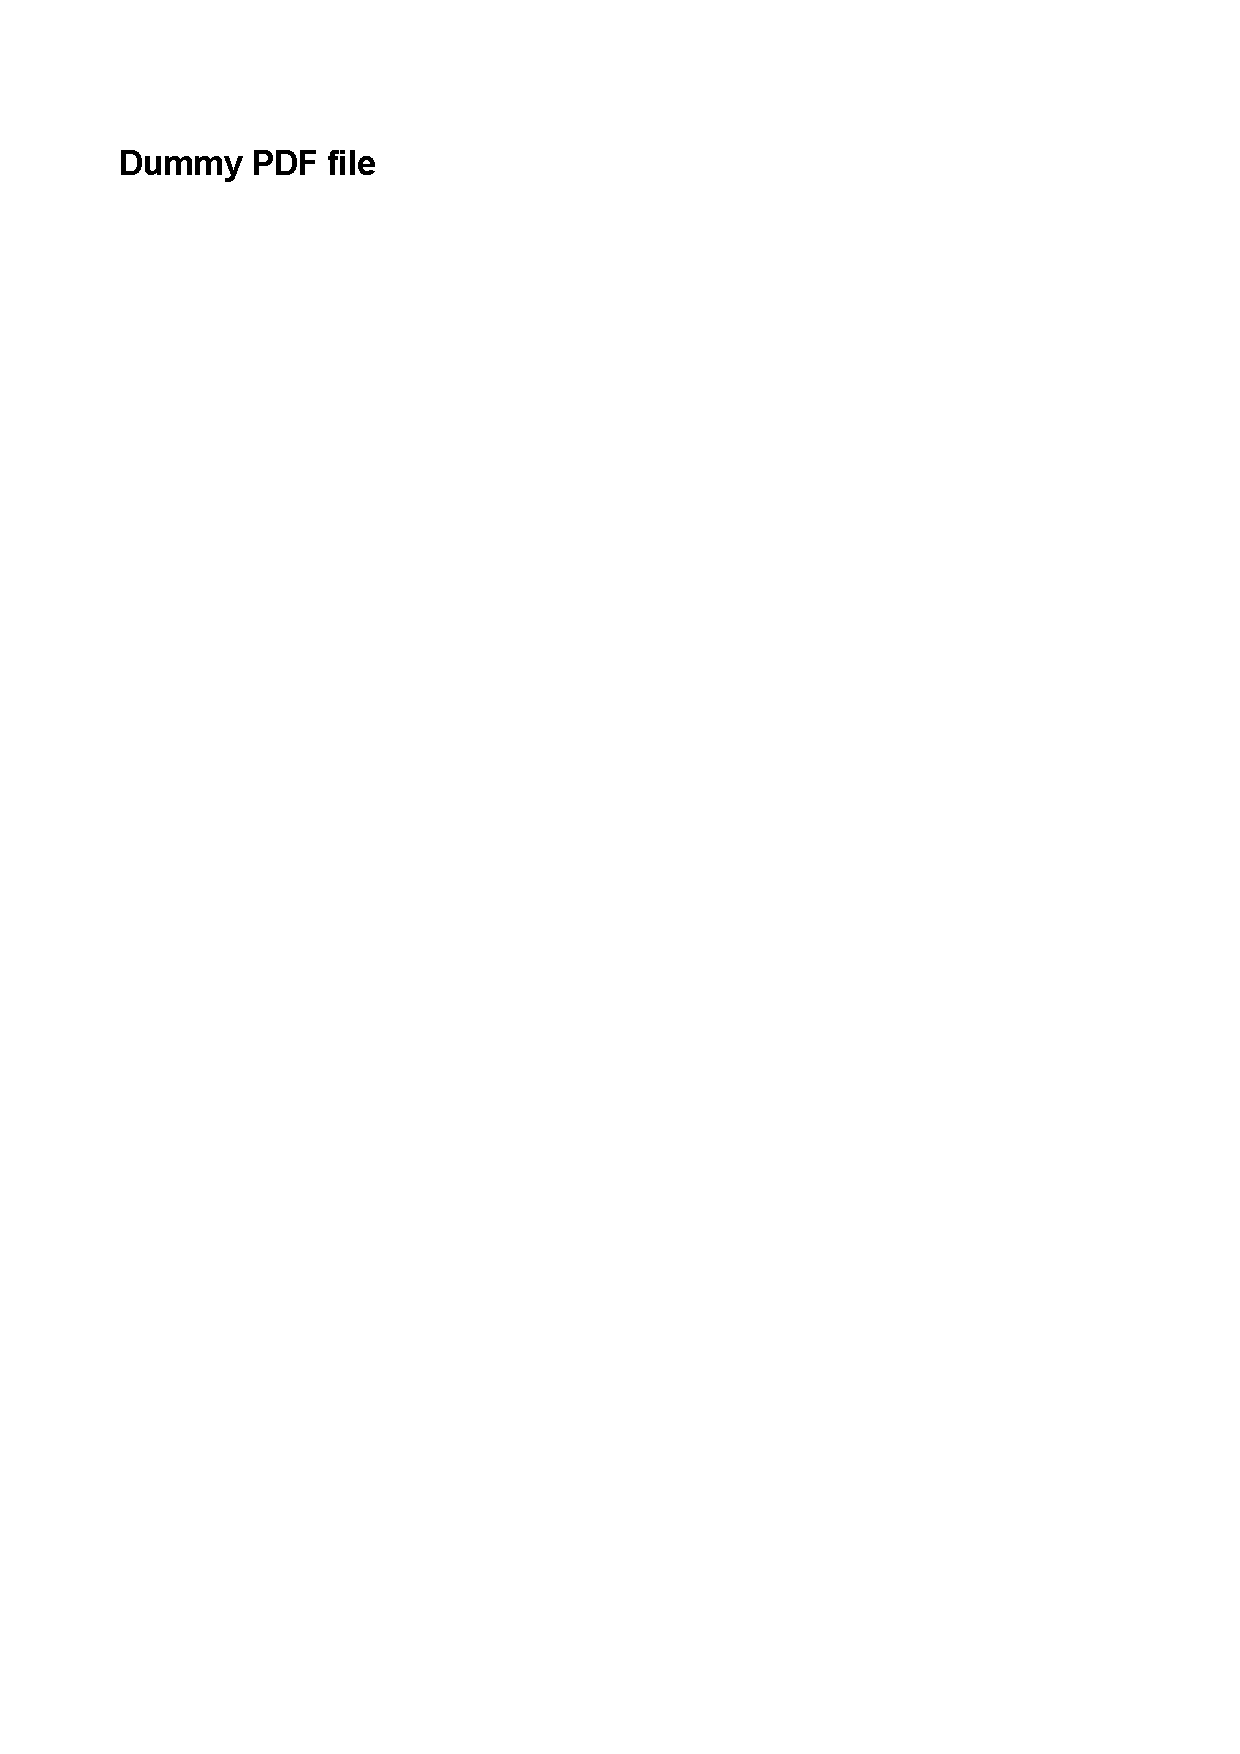
\includepdf[pages={-}]{pdf/dummy.pdf}

\end{document}
